% Options for packages loaded elsewhere
\PassOptionsToPackage{unicode}{hyperref}
\PassOptionsToPackage{hyphens}{url}
\PassOptionsToPackage{dvipsnames,svgnames,x11names}{xcolor}
%
\documentclass[
]{book}
\usepackage{amsmath,amssymb}
\usepackage{iftex}
\ifPDFTeX
  \usepackage[T1]{fontenc}
  \usepackage[utf8]{inputenc}
  \usepackage{textcomp} % provide euro and other symbols
\else % if luatex or xetex
  \usepackage{unicode-math} % this also loads fontspec
  \defaultfontfeatures{Scale=MatchLowercase}
  \defaultfontfeatures[\rmfamily]{Ligatures=TeX,Scale=1}
\fi
\usepackage{lmodern}
\ifPDFTeX\else
  % xetex/luatex font selection
\fi
% Use upquote if available, for straight quotes in verbatim environments
\IfFileExists{upquote.sty}{\usepackage{upquote}}{}
\IfFileExists{microtype.sty}{% use microtype if available
  \usepackage[]{microtype}
  \UseMicrotypeSet[protrusion]{basicmath} % disable protrusion for tt fonts
}{}
\makeatletter
\@ifundefined{KOMAClassName}{% if non-KOMA class
  \IfFileExists{parskip.sty}{%
    \usepackage{parskip}
  }{% else
    \setlength{\parindent}{0pt}
    \setlength{\parskip}{6pt plus 2pt minus 1pt}}
}{% if KOMA class
  \KOMAoptions{parskip=half}}
\makeatother
\usepackage{xcolor}
\usepackage{color}
\usepackage{fancyvrb}
\newcommand{\VerbBar}{|}
\newcommand{\VERB}{\Verb[commandchars=\\\{\}]}
\DefineVerbatimEnvironment{Highlighting}{Verbatim}{commandchars=\\\{\}}
% Add ',fontsize=\small' for more characters per line
\usepackage{framed}
\definecolor{shadecolor}{RGB}{248,248,248}
\newenvironment{Shaded}{\begin{snugshade}}{\end{snugshade}}
\newcommand{\AlertTok}[1]{\textcolor[rgb]{0.94,0.16,0.16}{#1}}
\newcommand{\AnnotationTok}[1]{\textcolor[rgb]{0.56,0.35,0.01}{\textbf{\textit{#1}}}}
\newcommand{\AttributeTok}[1]{\textcolor[rgb]{0.13,0.29,0.53}{#1}}
\newcommand{\BaseNTok}[1]{\textcolor[rgb]{0.00,0.00,0.81}{#1}}
\newcommand{\BuiltInTok}[1]{#1}
\newcommand{\CharTok}[1]{\textcolor[rgb]{0.31,0.60,0.02}{#1}}
\newcommand{\CommentTok}[1]{\textcolor[rgb]{0.56,0.35,0.01}{\textit{#1}}}
\newcommand{\CommentVarTok}[1]{\textcolor[rgb]{0.56,0.35,0.01}{\textbf{\textit{#1}}}}
\newcommand{\ConstantTok}[1]{\textcolor[rgb]{0.56,0.35,0.01}{#1}}
\newcommand{\ControlFlowTok}[1]{\textcolor[rgb]{0.13,0.29,0.53}{\textbf{#1}}}
\newcommand{\DataTypeTok}[1]{\textcolor[rgb]{0.13,0.29,0.53}{#1}}
\newcommand{\DecValTok}[1]{\textcolor[rgb]{0.00,0.00,0.81}{#1}}
\newcommand{\DocumentationTok}[1]{\textcolor[rgb]{0.56,0.35,0.01}{\textbf{\textit{#1}}}}
\newcommand{\ErrorTok}[1]{\textcolor[rgb]{0.64,0.00,0.00}{\textbf{#1}}}
\newcommand{\ExtensionTok}[1]{#1}
\newcommand{\FloatTok}[1]{\textcolor[rgb]{0.00,0.00,0.81}{#1}}
\newcommand{\FunctionTok}[1]{\textcolor[rgb]{0.13,0.29,0.53}{\textbf{#1}}}
\newcommand{\ImportTok}[1]{#1}
\newcommand{\InformationTok}[1]{\textcolor[rgb]{0.56,0.35,0.01}{\textbf{\textit{#1}}}}
\newcommand{\KeywordTok}[1]{\textcolor[rgb]{0.13,0.29,0.53}{\textbf{#1}}}
\newcommand{\NormalTok}[1]{#1}
\newcommand{\OperatorTok}[1]{\textcolor[rgb]{0.81,0.36,0.00}{\textbf{#1}}}
\newcommand{\OtherTok}[1]{\textcolor[rgb]{0.56,0.35,0.01}{#1}}
\newcommand{\PreprocessorTok}[1]{\textcolor[rgb]{0.56,0.35,0.01}{\textit{#1}}}
\newcommand{\RegionMarkerTok}[1]{#1}
\newcommand{\SpecialCharTok}[1]{\textcolor[rgb]{0.81,0.36,0.00}{\textbf{#1}}}
\newcommand{\SpecialStringTok}[1]{\textcolor[rgb]{0.31,0.60,0.02}{#1}}
\newcommand{\StringTok}[1]{\textcolor[rgb]{0.31,0.60,0.02}{#1}}
\newcommand{\VariableTok}[1]{\textcolor[rgb]{0.00,0.00,0.00}{#1}}
\newcommand{\VerbatimStringTok}[1]{\textcolor[rgb]{0.31,0.60,0.02}{#1}}
\newcommand{\WarningTok}[1]{\textcolor[rgb]{0.56,0.35,0.01}{\textbf{\textit{#1}}}}
\usepackage{longtable,booktabs,array}
\usepackage{calc} % for calculating minipage widths
% Correct order of tables after \paragraph or \subparagraph
\usepackage{etoolbox}
\makeatletter
\patchcmd\longtable{\par}{\if@noskipsec\mbox{}\fi\par}{}{}
\makeatother
% Allow footnotes in longtable head/foot
\IfFileExists{footnotehyper.sty}{\usepackage{footnotehyper}}{\usepackage{footnote}}
\makesavenoteenv{longtable}
\usepackage{graphicx}
\makeatletter
\def\maxwidth{\ifdim\Gin@nat@width>\linewidth\linewidth\else\Gin@nat@width\fi}
\def\maxheight{\ifdim\Gin@nat@height>\textheight\textheight\else\Gin@nat@height\fi}
\makeatother
% Scale images if necessary, so that they will not overflow the page
% margins by default, and it is still possible to overwrite the defaults
% using explicit options in \includegraphics[width, height, ...]{}
\setkeys{Gin}{width=\maxwidth,height=\maxheight,keepaspectratio}
% Set default figure placement to htbp
\makeatletter
\def\fps@figure{htbp}
\makeatother
\setlength{\emergencystretch}{3em} % prevent overfull lines
\providecommand{\tightlist}{%
  \setlength{\itemsep}{0pt}\setlength{\parskip}{0pt}}
\setcounter{secnumdepth}{5}
\usepackage{booktabs}
\usepackage{subfig}
\usepackage{booktabs}
\usepackage{longtable}
\usepackage{array}
\usepackage{multirow}
\usepackage{wrapfig}
\usepackage{float}
\usepackage{colortbl}
\usepackage{pdflscape}
\usepackage{tabu}
\usepackage{threeparttable}
\usepackage{threeparttablex}
\usepackage[normalem]{ulem}
\usepackage{makecell}
\usepackage{xcolor}
\ifLuaTeX
  \usepackage{selnolig}  % disable illegal ligatures
\fi
\usepackage[]{natbib}
\bibliographystyle{plainnat}
\IfFileExists{bookmark.sty}{\usepackage{bookmark}}{\usepackage{hyperref}}
\IfFileExists{xurl.sty}{\usepackage{xurl}}{} % add URL line breaks if available
\urlstyle{same}
\hypersetup{
  pdftitle={Visualizing NBA},
  pdfauthor={Junqi Fu},
  colorlinks=true,
  linkcolor={Maroon},
  filecolor={Maroon},
  citecolor={Blue},
  urlcolor={Blue},
  pdfcreator={LaTeX via pandoc}}

\title{Visualizing NBA}
\author{Junqi Fu}
\date{2023-10-21}

\begin{document}
\maketitle

{
\hypersetup{linkcolor=}
\setcounter{tocdepth}{2}
\tableofcontents
}
\hypertarget{nba-data}{%
\chapter{NBA Data}\label{nba-data}}

The data set contains all the players' performance data from season 1996-97 to season 2022-23.

\hypertarget{data-type}{%
\section{Data Type}\label{data-type}}

Here's a brief explanation of some important variable in the analysis:

\begin{itemize}
\tightlist
\item
  \textbf{player\_height}: player's height in the given season.
\item
  \textbf{player\_weight}: player's weight in the given season.
\item
  \textbf{gp}: total games a player has played in the given season.
\item
  \textbf{pts}: player's average points per game.
\item
  \textbf{reb}: player's average rebound per game.
\item
  \textbf{ast}: player's average assist per game.
\item
  \textbf{net\_rating}: the team's point differential per 100 possessions while a player is on court.
\item
  \textbf{oreb\_pct}: offensive rebound percentage - an estimate of the percentage of available offensive rebounds a player grabbed.
\item
  \textbf{dreb\_pct}: defensive rebound percentage - an estimate of the percentage of available defensive rebounds a player grabbed.
\item
  \textbf{usg\_pct}: usage percentage - an estimate of the percentage of team plays used by a player.
\item
  \textbf{ts\_pct}: true shooting percentage - a measure of shooting efficiency that takes into account field goals, 3-point field goals, and free throws.
\item
  \textbf{ast\_pct}: assist percentage - an estimate of the percentage of teammate field goals a player assisted.
\item
  \textbf{season}: season - the NBA season for which these stats apply.
\end{itemize}

\hypertarget{preliminary-cleaning}{%
\section{Preliminary Cleaning}\label{preliminary-cleaning}}

\hypertarget{initial-missing-data-imputation}{%
\subsection{Initial Missing Data Imputation}\label{initial-missing-data-imputation}}

\begin{Shaded}
\begin{Highlighting}[]
\FunctionTok{sum}\NormalTok{(}\FunctionTok{is.na}\NormalTok{(nba))}
\end{Highlighting}
\end{Shaded}

\begin{verbatim}
## [1] 0
\end{verbatim}

\begin{Shaded}
\begin{Highlighting}[]
\FunctionTok{md.pattern}\NormalTok{(nba)}
\end{Highlighting}
\end{Shaded}

\begin{verbatim}
##  /\     /\
## {  `---'  }
## {  O   O  }
## ==>  V <==  No need for mice. This data set is completely observed.
##  \  \|/  /
##   `-----'
\end{verbatim}

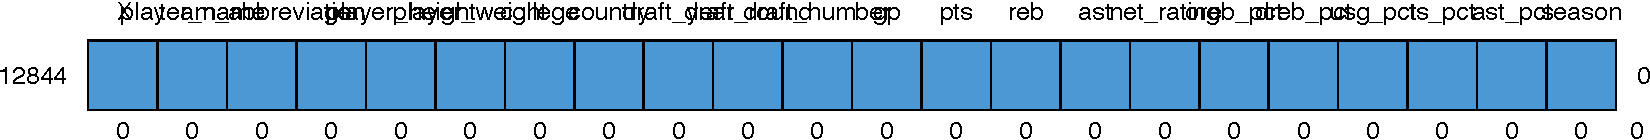
\includegraphics{NBA_Visualizing_files/figure-latex/unnamed-chunk-3-1.pdf}

\begin{verbatim}
##       X player_name team_abbreviation age player_height player_weight college
## 12844 1           1                 1   1             1             1       1
##       0           0                 0   0             0             0       0
##       country draft_year draft_round draft_number gp pts reb ast net_rating
## 12844       1          1           1            1  1   1   1   1          1
##             0          0           0            0  0   0   0   0          0
##       oreb_pct dreb_pct usg_pct ts_pct ast_pct season  
## 12844        1        1       1      1       1      1 0
##              0        0       0      0       0      0 0
\end{verbatim}

\begin{Shaded}
\begin{Highlighting}[]
\FunctionTok{md.pattern}\NormalTok{(}\FunctionTok{subset}\NormalTok{(nba, }\AttributeTok{select =} \FunctionTok{c}\NormalTok{(player\_height,}
\NormalTok{    player\_weight, gp, pts, reb, ast, net\_rating)))}
\end{Highlighting}
\end{Shaded}

\begin{verbatim}
##  /\     /\
## {  `---'  }
## {  O   O  }
## ==>  V <==  No need for mice. This data set is completely observed.
##  \  \|/  /
##   `-----'
\end{verbatim}

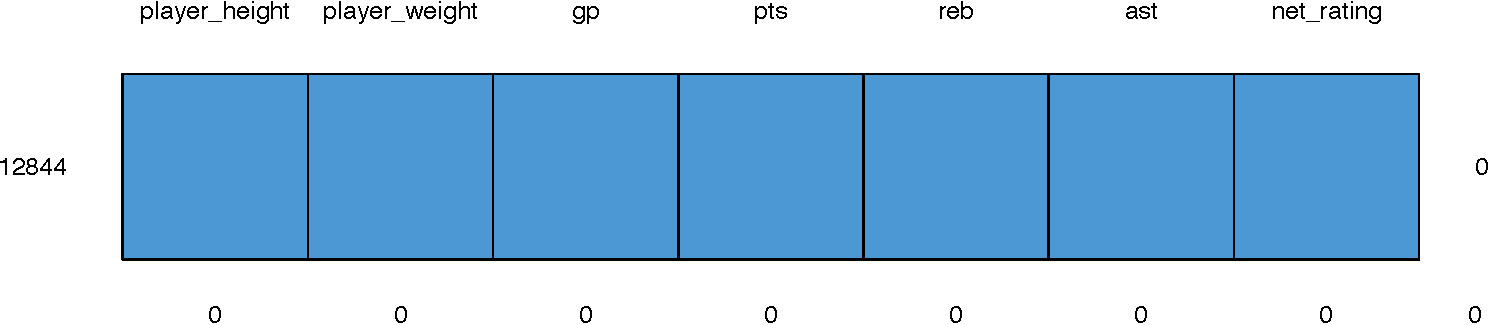
\includegraphics{NBA_Visualizing_files/figure-latex/unnamed-chunk-3-2.pdf}

\begin{verbatim}
##       player_height player_weight gp pts reb ast net_rating  
## 12844             1             1  1   1   1   1          1 0
##                   0             0  0   0   0   0          0 0
\end{verbatim}

\begin{Shaded}
\begin{Highlighting}[]
\FunctionTok{aggr}\NormalTok{(}\FunctionTok{subset}\NormalTok{(nba, }\AttributeTok{select =} \FunctionTok{c}\NormalTok{(player\_height,}
\NormalTok{    player\_weight, gp, pts, reb, ast, net\_rating)),}
    \AttributeTok{prop =}\NormalTok{ F, }\AttributeTok{numbers =} \ConstantTok{TRUE}\NormalTok{)}
\end{Highlighting}
\end{Shaded}

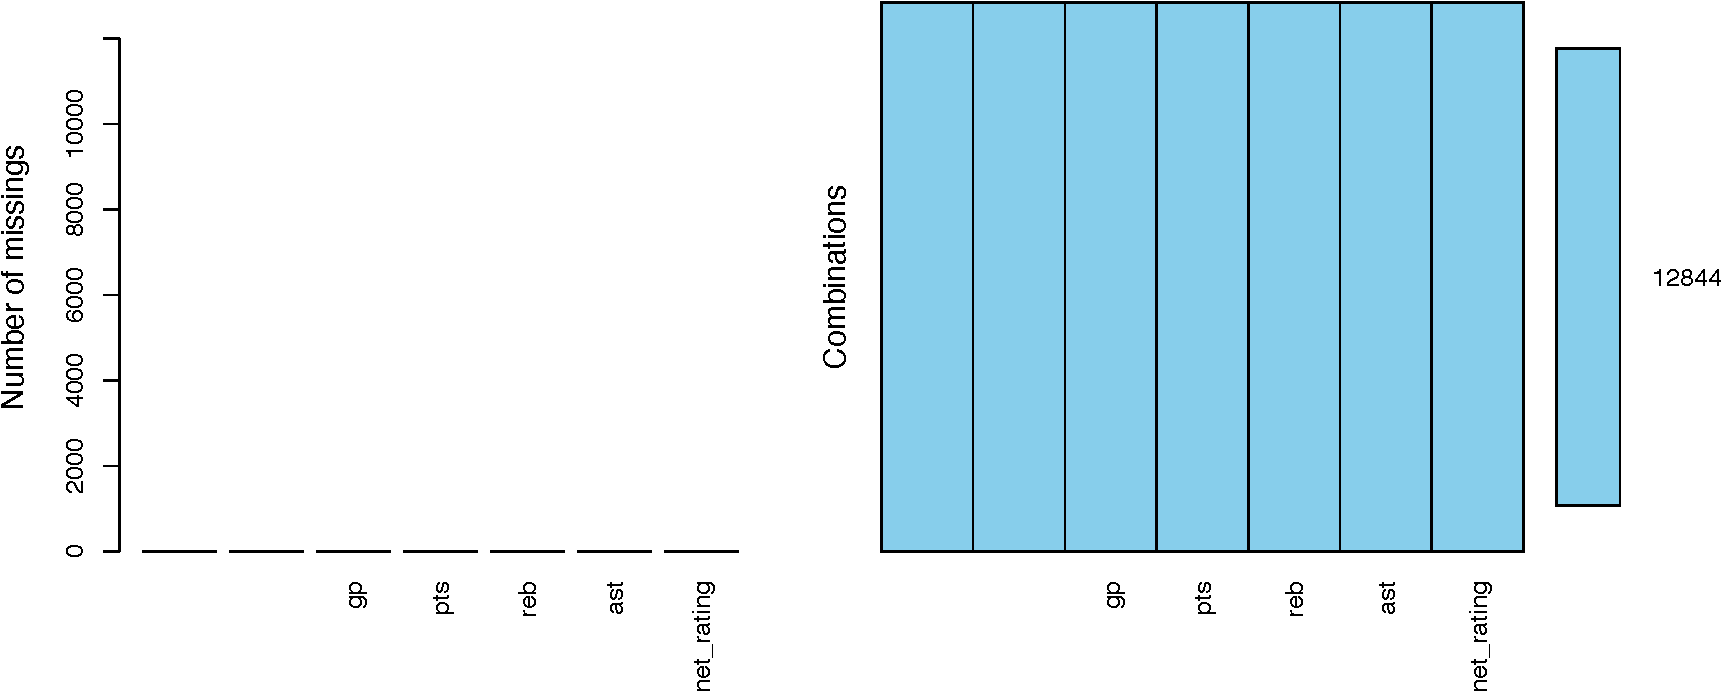
\includegraphics{NBA_Visualizing_files/figure-latex/unnamed-chunk-3-3.pdf}

\hypertarget{data-cleaning}{%
\subsection{Data Cleaning}\label{data-cleaning}}

identify outlier exists in the net\_rating, with the 300 as the max and -250 as the min.

\begin{Shaded}
\begin{Highlighting}[]
\FunctionTok{summary}\NormalTok{(nba)}
\end{Highlighting}
\end{Shaded}

\begin{verbatim}
##        X         player_name        team_abbreviation       age       
##  Min.   :    0   Length:12844       Length:12844       Min.   :18.00  
##  1st Qu.: 3211   Class :character   Class :character   1st Qu.:24.00  
##  Median : 6422   Mode  :character   Mode  :character   Median :26.00  
##  Mean   : 6422                                         Mean   :27.05  
##  3rd Qu.: 9632                                         3rd Qu.:30.00  
##  Max.   :12843                                         Max.   :44.00  
##  player_height   player_weight      college            country         
##  Min.   :160.0   Min.   : 60.33   Length:12844       Length:12844      
##  1st Qu.:193.0   1st Qu.: 90.72   Class :character   Class :character  
##  Median :200.7   Median : 99.79   Mode  :character   Mode  :character  
##  Mean   :200.6   Mean   :100.26                                        
##  3rd Qu.:208.3   3rd Qu.:108.86                                        
##  Max.   :231.1   Max.   :163.29                                        
##   draft_year        draft_round        draft_number             gp       
##  Length:12844       Length:12844       Length:12844       Min.   : 1.00  
##  Class :character   Class :character   Class :character   1st Qu.:31.00  
##  Mode  :character   Mode  :character   Mode  :character   Median :57.00  
##                                                           Mean   :51.15  
##                                                           3rd Qu.:73.00  
##                                                           Max.   :85.00  
##       pts              reb              ast           net_rating      
##  Min.   : 0.000   Min.   : 0.000   Min.   : 0.000   Min.   :-250.000  
##  1st Qu.: 3.600   1st Qu.: 1.800   1st Qu.: 0.600   1st Qu.:  -6.400  
##  Median : 6.700   Median : 3.000   Median : 1.200   Median :  -1.300  
##  Mean   : 8.213   Mean   : 3.558   Mean   : 1.825   Mean   :  -2.226  
##  3rd Qu.:11.500   3rd Qu.: 4.700   3rd Qu.: 2.400   3rd Qu.:   3.200  
##  Max.   :36.100   Max.   :16.300   Max.   :11.700   Max.   : 300.000  
##     oreb_pct          dreb_pct         usg_pct           ts_pct      
##  Min.   :0.00000   Min.   :0.0000   Min.   :0.0000   Min.   :0.0000  
##  1st Qu.:0.02100   1st Qu.:0.0960   1st Qu.:0.1490   1st Qu.:0.4820  
##  Median :0.04000   Median :0.1305   Median :0.1810   Median :0.5250  
##  Mean   :0.05407   Mean   :0.1406   Mean   :0.1846   Mean   :0.5131  
##  3rd Qu.:0.08300   3rd Qu.:0.1790   3rd Qu.:0.2170   3rd Qu.:0.5630  
##  Max.   :1.00000   Max.   :1.0000   Max.   :1.0000   Max.   :1.5000  
##     ast_pct          season         
##  Min.   :0.0000   Length:12844      
##  1st Qu.:0.0660   Class :character  
##  Median :0.1030   Mode  :character  
##  Mean   :0.1316                     
##  3rd Qu.:0.1790                     
##  Max.   :1.0000
\end{verbatim}

\begin{Shaded}
\begin{Highlighting}[]
\NormalTok{nba\_clean }\OtherTok{\textless{}{-}}\NormalTok{ (}\FunctionTok{which}\NormalTok{(nba}\SpecialCharTok{$}\NormalTok{net\_rating }\SpecialCharTok{\textgreater{}=} \DecValTok{300} \SpecialCharTok{|}
\NormalTok{    nba}\SpecialCharTok{$}\NormalTok{net\_rating }\SpecialCharTok{\textless{}=} \SpecialCharTok{{-}}\DecValTok{200}\NormalTok{))}
\NormalTok{nba }\OtherTok{\textless{}{-}}\NormalTok{ nba[}\SpecialCharTok{{-}}\NormalTok{nba\_clean]  }\CommentTok{\#remove the outliers.}
\end{Highlighting}
\end{Shaded}

\hypertarget{preliminary-descriptive-statistics}{%
\section{Preliminary Descriptive Statistics}\label{preliminary-descriptive-statistics}}

\begin{itemize}
\tightlist
\item
  \textbf{age}: the range is between a minimum of 18 years and a maximum of 44 years, with the average age being 26 years old.
\end{itemize}

\begin{Shaded}
\begin{Highlighting}[]
\FunctionTok{summary}\NormalTok{(nba}\SpecialCharTok{$}\NormalTok{age)}
\end{Highlighting}
\end{Shaded}

\begin{verbatim}
##    Min. 1st Qu.  Median    Mean 3rd Qu.    Max. 
##   18.00   24.00   26.00   27.05   30.00   44.00
\end{verbatim}

\begin{itemize}
\tightlist
\item
  \textbf{height}: the range is between a minimum of 160 cm and a maximum of 231.1 cm, with the average height as 200.7 cm.
\end{itemize}

\begin{Shaded}
\begin{Highlighting}[]
\FunctionTok{summary}\NormalTok{(nba}\SpecialCharTok{$}\NormalTok{player\_height)}
\end{Highlighting}
\end{Shaded}

\begin{verbatim}
##    Min. 1st Qu.  Median    Mean 3rd Qu.    Max. 
##   160.0   193.0   200.7   200.6   208.3   231.1
\end{verbatim}

\begin{itemize}
\tightlist
\item
  \textbf{weight}: the range is between a minimum of 60.33 kg and a maximum of 163.29 kg, with the average as 100 kg.
\end{itemize}

\begin{Shaded}
\begin{Highlighting}[]
\FunctionTok{summary}\NormalTok{(nba}\SpecialCharTok{$}\NormalTok{player\_weight)}
\end{Highlighting}
\end{Shaded}

\begin{verbatim}
##    Min. 1st Qu.  Median    Mean 3rd Qu.    Max. 
##   60.33   90.72   99.79  100.26  108.86  163.29
\end{verbatim}

\begin{itemize}
\tightlist
\item
  \textbf{player}: with a highly competitive threshold, only 2551 players have played in the league since 1996.
\end{itemize}

\begin{Shaded}
\begin{Highlighting}[]
\FunctionTok{summary}\NormalTok{(}\FunctionTok{unique}\NormalTok{(nba}\SpecialCharTok{$}\NormalTok{player\_name))}
\end{Highlighting}
\end{Shaded}

\begin{verbatim}
##    Length     Class      Mode 
##      2551 character character
\end{verbatim}

\hypertarget{hypothesis}{%
\chapter{Hypothesis}\label{hypothesis}}

\hypertarget{density-plot-for-height-and-weight}{%
\section{Density Plot for Height and Weight}\label{density-plot-for-height-and-weight}}

\hypertarget{density-plot-for-height-distribution-over-seasons}{%
\subsection{Density Plot for Height Distribution Over Seasons}\label{density-plot-for-height-distribution-over-seasons}}

\begin{Shaded}
\begin{Highlighting}[]
\NormalTok{heightplot }\OtherTok{\textless{}{-}} \FunctionTok{ggplot}\NormalTok{(nba, }\FunctionTok{aes}\NormalTok{(}\AttributeTok{x =}\NormalTok{ player\_height)) }\SpecialCharTok{+}
    \FunctionTok{geom\_density}\NormalTok{(}\FunctionTok{aes}\NormalTok{(}\AttributeTok{fill =}\NormalTok{ season), }\AttributeTok{alpha =} \FloatTok{0.4}\NormalTok{) }\SpecialCharTok{+}
    \FunctionTok{geom\_vline}\NormalTok{(}\FunctionTok{aes}\NormalTok{(}\AttributeTok{xintercept =} \FunctionTok{mean}\NormalTok{(player\_height)),}
        \AttributeTok{linetype =} \StringTok{"dashed"}\NormalTok{, }\AttributeTok{color =} \StringTok{"red"}\NormalTok{) }\SpecialCharTok{+}
    \FunctionTok{ggtitle}\NormalTok{(}\StringTok{"Density Plot of Player Heights"}\NormalTok{) }\SpecialCharTok{+}
    \FunctionTok{xlab}\NormalTok{(}\StringTok{"Player Height (cm)"}\NormalTok{) }\SpecialCharTok{+} \FunctionTok{ylab}\NormalTok{(}\StringTok{"Density"}\NormalTok{) }\SpecialCharTok{+}
    \FunctionTok{theme\_minimal}\NormalTok{()}
\FunctionTok{print}\NormalTok{(heightplot)}
\end{Highlighting}
\end{Shaded}

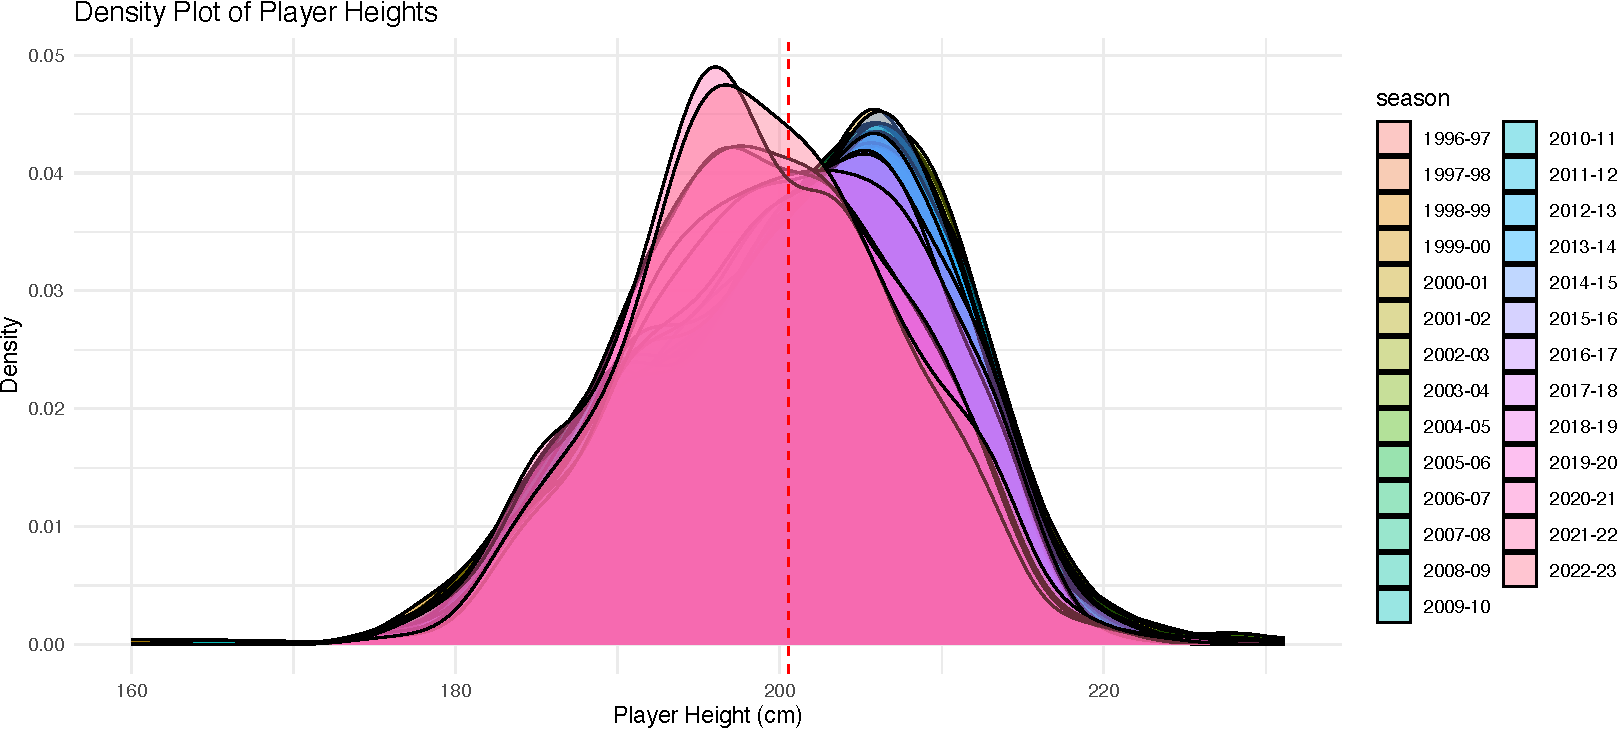
\includegraphics{NBA_Visualizing_files/figure-latex/unnamed-chunk-11-1.pdf}

\hypertarget{summary}{%
\subsubsection{Summary}\label{summary}}

\begin{itemize}
\item
  A more noticeable shift in the mean height of players over seasons. The mean height has decreased steadily.
\item
  A narrower range of heights among players in the recent NBA compared to the past.
\item
  There's a noticeable peak around the 200-210 cm range, suggesting that a significant number of players fall within this height bracket.
\end{itemize}

\hypertarget{density-plot-for-weight-distribution-over-seasons}{%
\subsection{Density Plot for Weight Distribution Over Seasons}\label{density-plot-for-weight-distribution-over-seasons}}

\begin{Shaded}
\begin{Highlighting}[]
\NormalTok{weightplot }\OtherTok{\textless{}{-}} \FunctionTok{ggplot}\NormalTok{(nba, }\FunctionTok{aes}\NormalTok{(}\AttributeTok{x =}\NormalTok{ player\_weight)) }\SpecialCharTok{+}
    \FunctionTok{geom\_density}\NormalTok{(}\FunctionTok{aes}\NormalTok{(}\AttributeTok{fill =}\NormalTok{ season), }\AttributeTok{alpha =} \FloatTok{0.4}\NormalTok{) }\SpecialCharTok{+}
    \FunctionTok{geom\_vline}\NormalTok{(}\FunctionTok{aes}\NormalTok{(}\AttributeTok{xintercept =} \FunctionTok{mean}\NormalTok{(player\_weight)),}
        \AttributeTok{linetype =} \StringTok{"dashed"}\NormalTok{, }\AttributeTok{color =} \StringTok{"red"}\NormalTok{) }\SpecialCharTok{+}
    \FunctionTok{ggtitle}\NormalTok{(}\StringTok{"Density Plot of Player Weights"}\NormalTok{) }\SpecialCharTok{+}
    \FunctionTok{xlab}\NormalTok{(}\StringTok{"Player Weight (kg)"}\NormalTok{) }\SpecialCharTok{+} \FunctionTok{ylab}\NormalTok{(}\StringTok{"Density"}\NormalTok{) }\SpecialCharTok{+}
    \FunctionTok{theme\_minimal}\NormalTok{()}
\FunctionTok{print}\NormalTok{(weightplot)}
\end{Highlighting}
\end{Shaded}

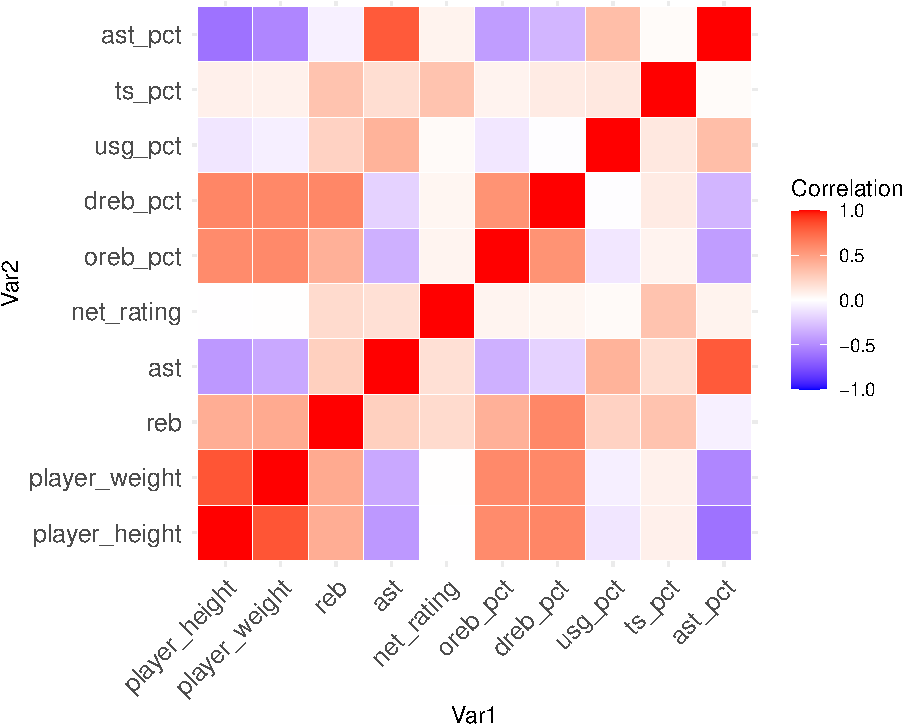
\includegraphics{NBA_Visualizing_files/figure-latex/unnamed-chunk-12-1.pdf}

\hypertarget{summary-1}{%
\subsubsection{Summary}\label{summary-1}}

\begin{itemize}
\tightlist
\item
  The mean weight seems to have shifted towards the left, suggesting that players have, on average, become lighter over the years.
\item
  The distributions for the recent seasons appear narrower, indicating less variability in player weights now than in earlier seasons.
\end{itemize}

\hypertarget{general-conclusion}{%
\subsection{General Conclusion}\label{general-conclusion}}

In summary, over the years, NBA players have, on average, become shorter and lighter, with a narrower range of both weights and heights represented in recent seasons.

\hypertarget{inference-hypothesis-based-on-the-density-plot-and-initial-summary}{%
\section{Inference \& Hypothesis Based On The Density Plot and Initial Summary}\label{inference-hypothesis-based-on-the-density-plot-and-initial-summary}}

\begin{itemize}
\item
  \textbf{H1} Versatility \& Position-less Basketball: the narrower range of heights and weights indicates that there might be an increasing trend of ``position-less'' basketball, specifically players are no longer strictly confined to traditional roles based on their physical attributes.
\item
  \textbf{H2} Evolution in Playing Style: the traditional center-focused style of play cannot adapt to the pace of the modern NBA.
\end{itemize}

\hypertarget{correlation-analysis}{%
\chapter{Correlation Analysis}\label{correlation-analysis}}

\hypertarget{correlation-between-hw-and-others}{%
\section{Correlation Between H/W and Others}\label{correlation-between-hw-and-others}}

\begin{itemize}
\tightlist
\item
  The correlation matrix visually represents the relationship between height/weight and other basketball metrics.
\item
  Correlations range between -1.0 and 1.0, with darker red indicating a strong positive correlation, blue indicating a strong negative correlation, and lighter shades (towards white) indicating weaker or no correlation.
\end{itemize}

\begin{Shaded}
\begin{Highlighting}[]
\FunctionTok{ggplot}\NormalTok{(}\AttributeTok{data =}\NormalTok{ melted\_cormat, }\FunctionTok{aes}\NormalTok{(}\AttributeTok{x =}\NormalTok{ Var1,}
    \AttributeTok{y =}\NormalTok{ Var2)) }\SpecialCharTok{+} \FunctionTok{geom\_tile}\NormalTok{(}\FunctionTok{aes}\NormalTok{(}\AttributeTok{fill =}\NormalTok{ value),}
    \AttributeTok{color =} \StringTok{"white"}\NormalTok{) }\SpecialCharTok{+} \FunctionTok{scale\_fill\_gradient2}\NormalTok{(}\AttributeTok{low =} \StringTok{"blue"}\NormalTok{,}
    \AttributeTok{high =} \StringTok{"red"}\NormalTok{, }\AttributeTok{mid =} \StringTok{"white"}\NormalTok{, }\AttributeTok{midpoint =} \DecValTok{0}\NormalTok{,}
    \AttributeTok{limit =} \FunctionTok{c}\NormalTok{(}\SpecialCharTok{{-}}\DecValTok{1}\NormalTok{, }\DecValTok{1}\NormalTok{), }\AttributeTok{space =} \StringTok{"Lab"}\NormalTok{, }\AttributeTok{name =} \StringTok{"Correlation"}\NormalTok{) }\SpecialCharTok{+}
    \FunctionTok{theme\_minimal}\NormalTok{() }\SpecialCharTok{+} \FunctionTok{theme}\NormalTok{(}\AttributeTok{axis.text.x =} \FunctionTok{element\_text}\NormalTok{(}\AttributeTok{angle =} \DecValTok{45}\NormalTok{,}
    \AttributeTok{vjust =} \DecValTok{1}\NormalTok{, }\AttributeTok{size =} \DecValTok{12}\NormalTok{, }\AttributeTok{hjust =} \DecValTok{1}\NormalTok{), }\AttributeTok{axis.text.y =} \FunctionTok{element\_text}\NormalTok{(}\AttributeTok{size =} \DecValTok{12}\NormalTok{)) }\SpecialCharTok{+}
    \FunctionTok{coord\_fixed}\NormalTok{()}
\end{Highlighting}
\end{Shaded}

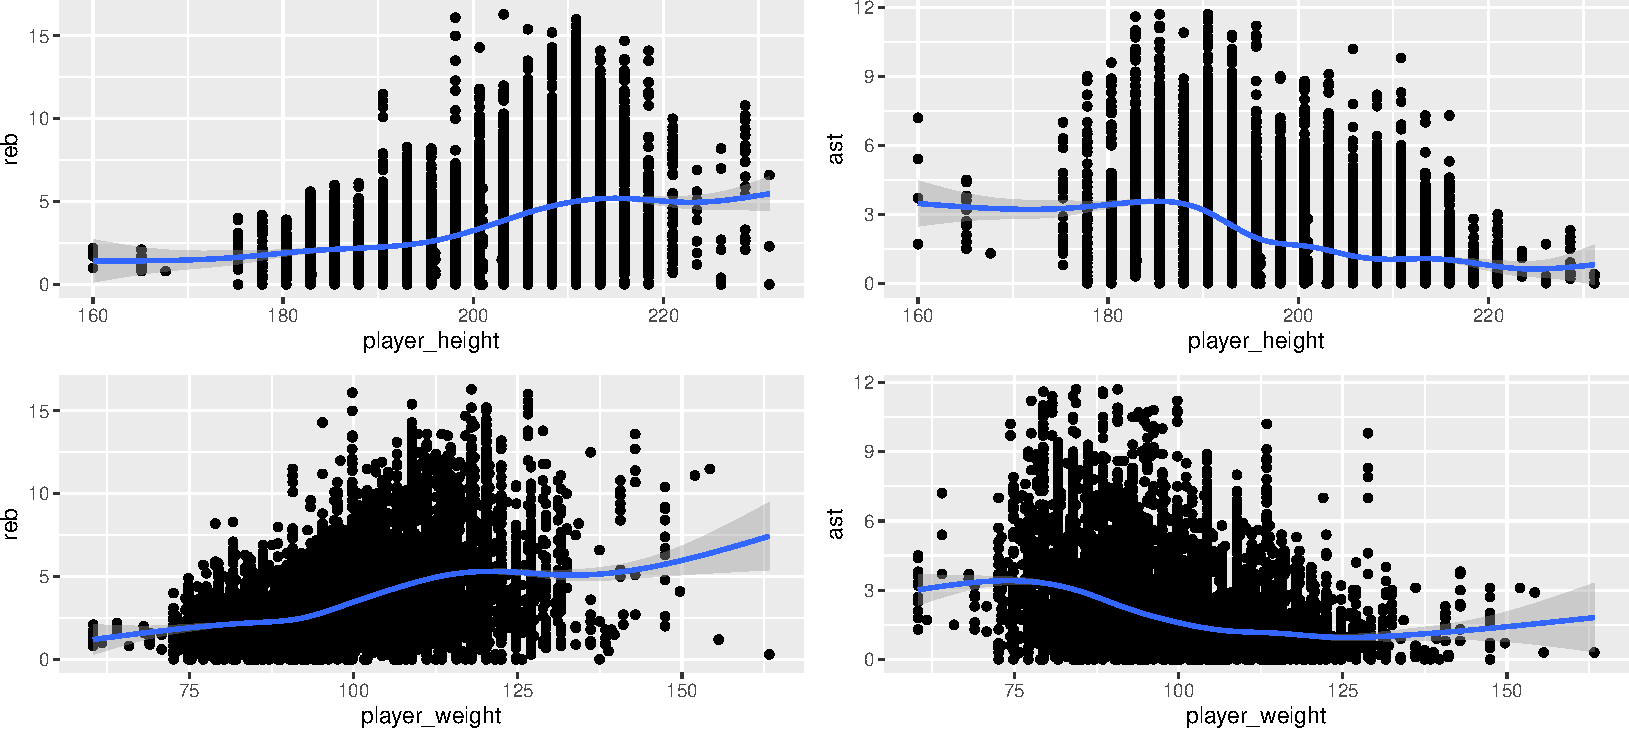
\includegraphics{NBA_Visualizing_files/figure-latex/unnamed-chunk-14-1.pdf}

\hypertarget{correlation-matrix}{%
\section{Correlation Matrix}\label{correlation-matrix}}

\begin{itemize}
\tightlist
\item
  A strong positive correlation between height and defensive rebound percentage as well as offensive rebound percentage.
\item
  Weight also shows positive correlations with both rebound percentage, though slightly weaker compared to height.
\item
  Height seems to have a negative correlation with assist percentage, suggesting taller players might assist less.
\item
  Other metrics like true shooting percentage and usage percentage have weaker correlations with height and weight.
\end{itemize}

\hypertarget{correlation-between-hw-and-ra}{%
\section{Correlation Between H/W and R/A}\label{correlation-between-hw-and-ra}}

Four scatter plots depict the relationships between player height, player weight, rebounds, and assists.

\begin{Shaded}
\begin{Highlighting}[]
\NormalTok{height\_reb }\OtherTok{\textless{}{-}} \FunctionTok{ggplot}\NormalTok{(nba, }\FunctionTok{aes}\NormalTok{(}\AttributeTok{x =}\NormalTok{ player\_height,}
    \AttributeTok{y =}\NormalTok{ reb))}
\NormalTok{height\_reb }\OtherTok{\textless{}{-}}\NormalTok{ height\_reb }\SpecialCharTok{+} \FunctionTok{geom\_point}\NormalTok{()}

\NormalTok{height\_ast }\OtherTok{\textless{}{-}} \FunctionTok{ggplot}\NormalTok{(nba, }\FunctionTok{aes}\NormalTok{(}\AttributeTok{x =}\NormalTok{ player\_height,}
    \AttributeTok{y =}\NormalTok{ ast))}
\NormalTok{height\_ast }\OtherTok{\textless{}{-}}\NormalTok{ height\_ast }\SpecialCharTok{+} \FunctionTok{geom\_point}\NormalTok{()}

\NormalTok{weight\_reb }\OtherTok{\textless{}{-}} \FunctionTok{ggplot}\NormalTok{(nba, }\FunctionTok{aes}\NormalTok{(}\AttributeTok{x =}\NormalTok{ player\_weight,}
    \AttributeTok{y =}\NormalTok{ reb))}
\NormalTok{weight\_reb }\OtherTok{\textless{}{-}}\NormalTok{ weight\_reb }\SpecialCharTok{+} \FunctionTok{geom\_point}\NormalTok{()}

\NormalTok{weight\_ast }\OtherTok{\textless{}{-}} \FunctionTok{ggplot}\NormalTok{(nba, }\FunctionTok{aes}\NormalTok{(}\AttributeTok{x =}\NormalTok{ player\_weight,}
    \AttributeTok{y =}\NormalTok{ ast))}
\NormalTok{weight\_ast }\OtherTok{\textless{}{-}}\NormalTok{ weight\_ast }\SpecialCharTok{+} \FunctionTok{geom\_point}\NormalTok{()}
\end{Highlighting}
\end{Shaded}

\begin{Shaded}
\begin{Highlighting}[]
\FunctionTok{grid.arrange}\NormalTok{(height\_reb }\SpecialCharTok{+} \FunctionTok{geom\_smooth}\NormalTok{(),}
\NormalTok{    height\_ast }\SpecialCharTok{+} \FunctionTok{geom\_smooth}\NormalTok{(), weight\_reb }\SpecialCharTok{+}
        \FunctionTok{geom\_smooth}\NormalTok{(), weight\_ast }\SpecialCharTok{+} \FunctionTok{geom\_smooth}\NormalTok{(),}
    \AttributeTok{ncol =} \DecValTok{2}\NormalTok{)}
\end{Highlighting}
\end{Shaded}

\begin{verbatim}
## `geom_smooth()` using method = 'gam' and formula = 'y ~ s(x, bs = "cs")'
## `geom_smooth()` using method = 'gam' and formula = 'y ~ s(x, bs = "cs")'
## `geom_smooth()` using method = 'gam' and formula = 'y ~ s(x, bs = "cs")'
## `geom_smooth()` using method = 'gam' and formula = 'y ~ s(x, bs = "cs")'
\end{verbatim}

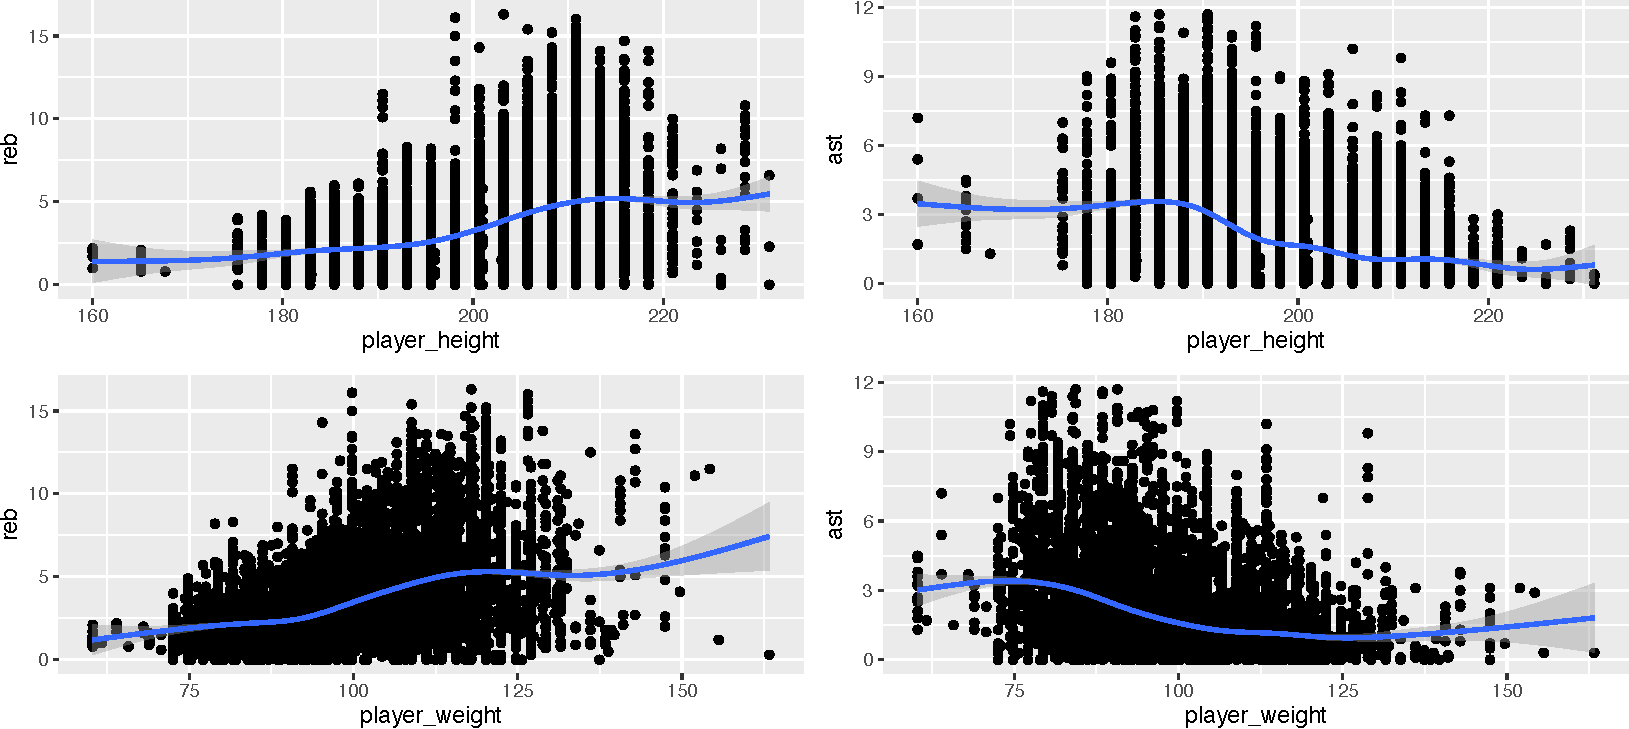
\includegraphics{NBA_Visualizing_files/figure-latex/unnamed-chunk-16-1.pdf}

\hypertarget{summary-from-scatter-plots}{%
\section{Summary From Scatter Plots}\label{summary-from-scatter-plots}}

\begin{itemize}
\tightlist
\item
  Consistent with the correlation matrix, height and rebound idsplays an upward trend, indicating that taller players tend to have more rebounds.
\item
  Conversely, height and assist depicts a downward trend, signifying that shorter players usually have more assists.
\end{itemize}

\hypertarget{net-rating-by-players-physical-attributes}{%
\section{Net Rating By Player's Physical Attributes}\label{net-rating-by-players-physical-attributes}}

The boxplots depict the distribution of net rating (i.e., the team's point differential per 100 possessions while a player is on court) across various player heights and weights.

\begin{Shaded}
\begin{Highlighting}[]
\NormalTok{heightdatapart }\OtherTok{\textless{}{-}} \FunctionTok{data.frame}\NormalTok{(}\AttributeTok{player\_height =}\NormalTok{ nba}\SpecialCharTok{$}\NormalTok{player\_height,}
    \AttributeTok{net\_rating =}\NormalTok{ nba}\SpecialCharTok{$}\NormalTok{net\_rating)}
\NormalTok{heightdatapart }\OtherTok{\textless{}{-}}\NormalTok{ heightdatapart[(heightdatapart}\SpecialCharTok{$}\NormalTok{net\_rating }\SpecialCharTok{\textgreater{}=}
    \SpecialCharTok{{-}}\DecValTok{50} \SpecialCharTok{\&}\NormalTok{ heightdatapart}\SpecialCharTok{$}\NormalTok{net\_rating }\SpecialCharTok{\textless{}=} \DecValTok{50}\NormalTok{),}
\NormalTok{    ]}
\NormalTok{heightdatapart}\SpecialCharTok{$}\NormalTok{group }\OtherTok{\textless{}{-}} \FunctionTok{cut}\NormalTok{(heightdatapart}\SpecialCharTok{$}\NormalTok{player\_height,}
    \AttributeTok{breaks =} \DecValTok{7}\NormalTok{)}
\NormalTok{ph }\OtherTok{\textless{}{-}} \FunctionTok{ggplot}\NormalTok{(}\AttributeTok{data =}\NormalTok{ heightdatapart, }\FunctionTok{aes}\NormalTok{(}\AttributeTok{x =}\NormalTok{ group,}
    \AttributeTok{y =}\NormalTok{ net\_rating, }\AttributeTok{fill =}\NormalTok{ group)) }\SpecialCharTok{+} \FunctionTok{geom\_boxplot}\NormalTok{() }\SpecialCharTok{+}
    \FunctionTok{ggtitle}\NormalTok{(}\StringTok{"Net Rating by Player Height"}\NormalTok{) }\SpecialCharTok{+}
    \FunctionTok{theme\_minimal}\NormalTok{()}
\FunctionTok{print}\NormalTok{(ph)}
\end{Highlighting}
\end{Shaded}

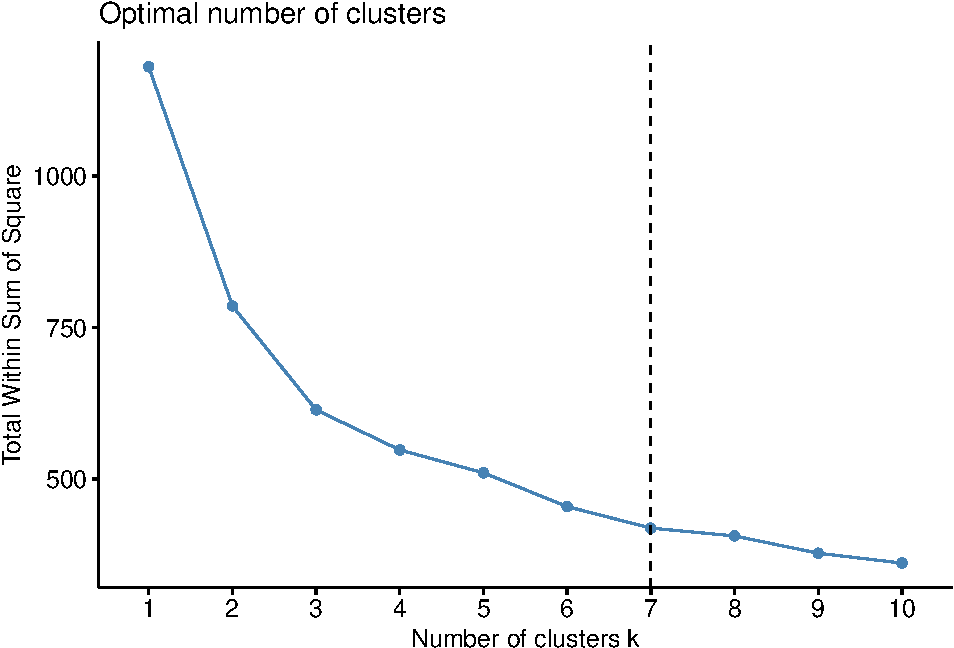
\includegraphics{NBA_Visualizing_files/figure-latex/unnamed-chunk-20-1.pdf}

\begin{Shaded}
\begin{Highlighting}[]
\NormalTok{weightdatapart }\OtherTok{\textless{}{-}} \FunctionTok{data.frame}\NormalTok{(}\AttributeTok{player\_weight =}\NormalTok{ nba}\SpecialCharTok{$}\NormalTok{player\_weight,}
    \AttributeTok{net\_rating =}\NormalTok{ nba}\SpecialCharTok{$}\NormalTok{net\_rating)}
\NormalTok{weightdatapart }\OtherTok{\textless{}{-}}\NormalTok{ weightdatapart[(weightdatapart}\SpecialCharTok{$}\NormalTok{net\_rating }\SpecialCharTok{\textgreater{}=}
    \SpecialCharTok{{-}}\DecValTok{50} \SpecialCharTok{\&}\NormalTok{ weightdatapart}\SpecialCharTok{$}\NormalTok{net\_rating }\SpecialCharTok{\textless{}=} \DecValTok{50}\NormalTok{),}
\NormalTok{    ]}
\NormalTok{weightdatapart}\SpecialCharTok{$}\NormalTok{group }\OtherTok{\textless{}{-}} \FunctionTok{cut}\NormalTok{(weightdatapart}\SpecialCharTok{$}\NormalTok{player\_weight,}
    \AttributeTok{breaks =} \DecValTok{7}\NormalTok{)}
\NormalTok{pw }\OtherTok{\textless{}{-}} \FunctionTok{ggplot}\NormalTok{(}\AttributeTok{data =}\NormalTok{ weightdatapart, }\FunctionTok{aes}\NormalTok{(}\AttributeTok{x =}\NormalTok{ group,}
    \AttributeTok{y =}\NormalTok{ net\_rating, }\AttributeTok{fill =}\NormalTok{ group)) }\SpecialCharTok{+} \FunctionTok{geom\_boxplot}\NormalTok{() }\SpecialCharTok{+}
    \FunctionTok{ggtitle}\NormalTok{(}\StringTok{"Net Rating by Player Weight"}\NormalTok{) }\SpecialCharTok{+}
    \FunctionTok{theme\_minimal}\NormalTok{()}
\FunctionTok{print}\NormalTok{(pw)}
\end{Highlighting}
\end{Shaded}

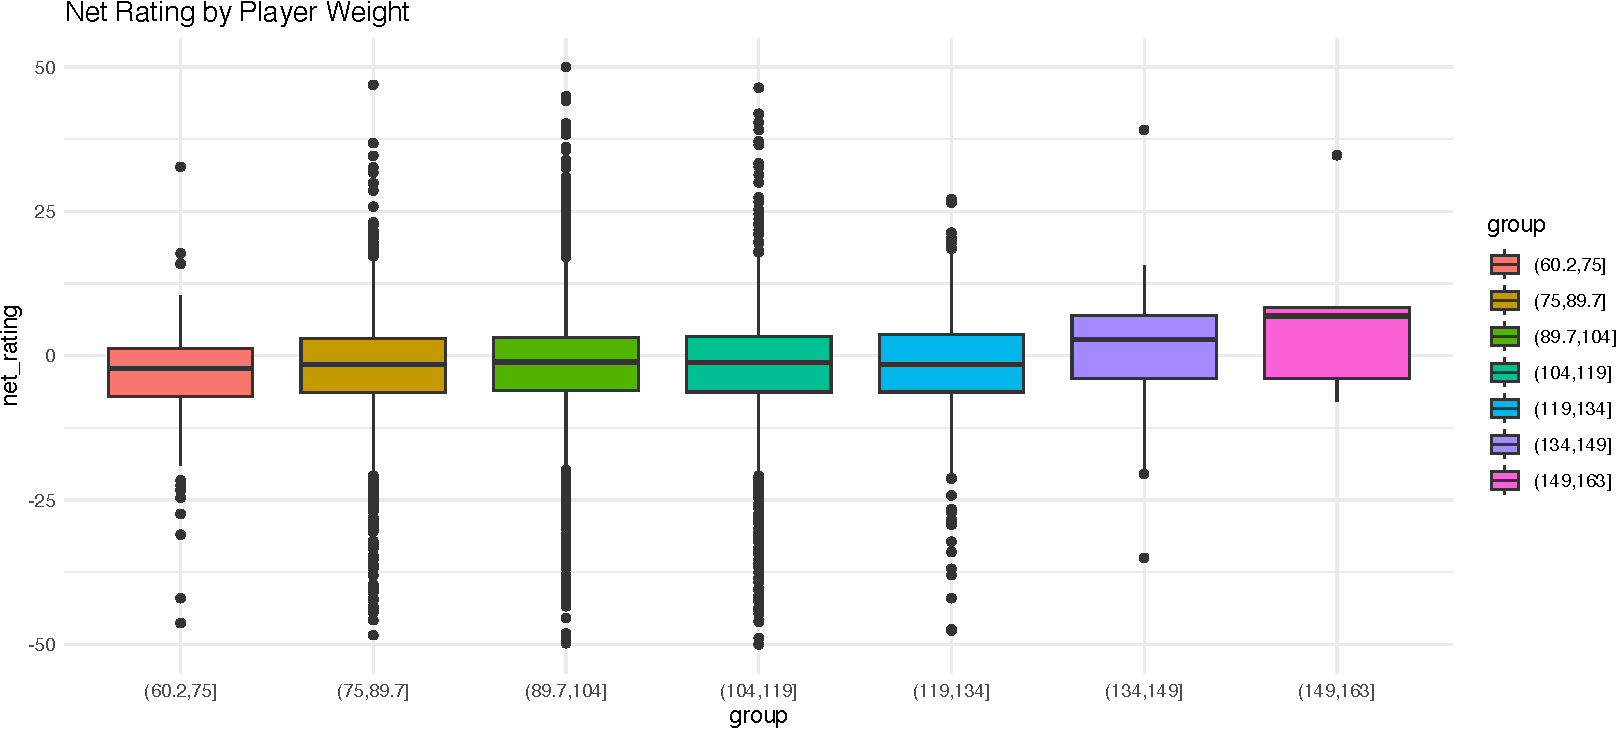
\includegraphics{NBA_Visualizing_files/figure-latex/unnamed-chunk-20-2.pdf}

\hypertarget{summary-from-box-plot}{%
\section{Summary From Box Plot}\label{summary-from-box-plot}}

\hypertarget{net-rating-by-player-height}{%
\subsection{Net Rating by Player Height}\label{net-rating-by-player-height}}

\begin{itemize}
\tightlist
\item
  Players in the height range of 190 cm to 203 cm tend to have a wider variation in net rating, with some players in this range even having exceptionally high net ratings.
\item
  Taller players, especially those between 206 cm and 211 cm, have a slightly lower median net rating.
\item
  The shorter players, particularly those below 188 cm, also show a lower median net rating, but with less variability than the taller players.
\item
  Players who are 213 cm and above exhibit a narrower interquartile range (middle 50\% of data) but with a few outliers having lower net ratings.
\end{itemize}

\hypertarget{net-rating-by-player-weight}{%
\subsection{Net Rating by Player Weight}\label{net-rating-by-player-weight}}

\begin{itemize}
\tightlist
\item
  Players weighing between 70-85 kg and 100-115 kg display a wider range in net rating, with some outliers, particularly on the higher end.
\item
  Players in the weight range of 85-100 kg have a median net rating that's slightly higher, with a more compact interquartile range, indicating less variability in their performance.
\item
  Heavier players, weighing 119 kg and above, exhibit a narrower interquartile range with a few lower outliers.
  From the boxplots, it can be concluded that:
\end{itemize}

\hypertarget{general-summary}{%
\subsection{General Summary}\label{general-summary}}

\begin{itemize}
\tightlist
\item
  Players of medium height (190 cm to 203 cm) tend to have varied performances, with some players being exceptionally good based on net rating.
\item
  The shortest and the tallest players tend to have a slightly lower median net rating.
\item
  Players of medium weight (85-100 kg) generally have consistent performances, while players on the lighter and heavier ends show greater variability in net rating.
\end{itemize}

\hypertarget{in-depth-analysis-for-hw}{%
\chapter{In-depth Analysis for H/W}\label{in-depth-analysis-for-hw}}

\hypertarget{what-can-be-answered-for-now}{%
\section{What Can Be Answered For Now?}\label{what-can-be-answered-for-now}}

\begin{itemize}
\item
  H1: Versatility \& Position-less Basketball
  Given the narrow range of heights and weights and the varied performance of players irrespective of their physical attributes, it does hint towards the emergence of ``position-less'' basketball. Players are breaking traditional molds, and their skills are no longer just confined to their height and weight.
\item
  H2: Evolution in Playing Style
  The NBA's pace and style have evolved, favoring versatile players over traditional roles. The varied performances of players, especially the medium-height ones, and the shift from a strong center-focused game further supports this hypothesis.
\end{itemize}

\begin{Shaded}
\begin{Highlighting}[]
\NormalTok{p1 }\OtherTok{\textless{}{-}} \FunctionTok{ggplot}\NormalTok{(nba, }\FunctionTok{aes}\NormalTok{(}\AttributeTok{x =}\NormalTok{ player\_weight,}
    \AttributeTok{y =}\NormalTok{ player\_height))}
\NormalTok{p1 }\OtherTok{\textless{}{-}}\NormalTok{ p1 }\SpecialCharTok{+} \FunctionTok{geom\_point}\NormalTok{()}
\NormalTok{p1 }\SpecialCharTok{+} \FunctionTok{geom\_smooth}\NormalTok{()}
\end{Highlighting}
\end{Shaded}

\begin{verbatim}
## `geom_smooth()` using method = 'gam' and formula = 'y ~ s(x, bs = "cs")'
\end{verbatim}

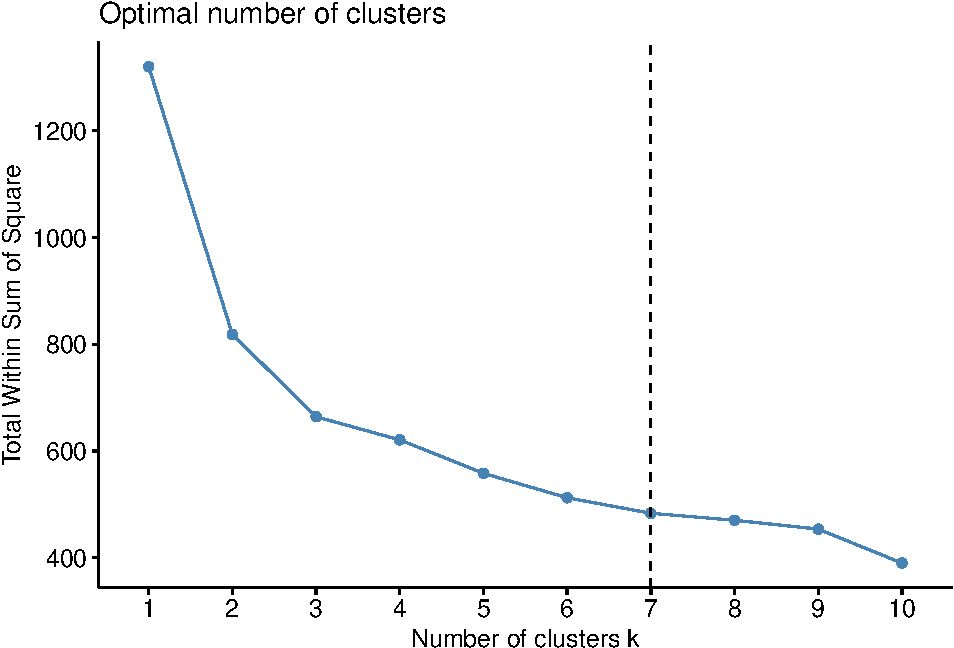
\includegraphics{NBA_Visualizing_files/figure-latex/unnamed-chunk-22-1.pdf}

\hypertarget{time-series-visualization}{%
\section{Time-series Visualization}\label{time-series-visualization}}

To further explore H1 and H2, a time-series analysis portraying the fluctuating correlation between height and weight over seasons has been drawn.

\begin{Shaded}
\begin{Highlighting}[]
\NormalTok{p }\OtherTok{\textless{}{-}} \FunctionTok{ggplot}\NormalTok{(cor\_df, }\FunctionTok{aes}\NormalTok{(}\AttributeTok{x =}\NormalTok{ season,}
    \AttributeTok{y =}\NormalTok{ correlation,}
    \AttributeTok{group =} \DecValTok{1}\NormalTok{)) }\SpecialCharTok{+} \FunctionTok{geom\_line}\NormalTok{() }\SpecialCharTok{+}
    \FunctionTok{xlab}\NormalTok{(}\StringTok{"Season"}\NormalTok{) }\SpecialCharTok{+}
    \FunctionTok{ylab}\NormalTok{(}\StringTok{"Correlation between Height and Weight"}\NormalTok{) }\SpecialCharTok{+}
    \FunctionTok{ggtitle}\NormalTok{(}\StringTok{"Correlation between Height and Weight over Seasons"}\NormalTok{) }\SpecialCharTok{+}
    \FunctionTok{theme\_minimal}\NormalTok{()}
\FunctionTok{print}\NormalTok{(p)}
\end{Highlighting}
\end{Shaded}

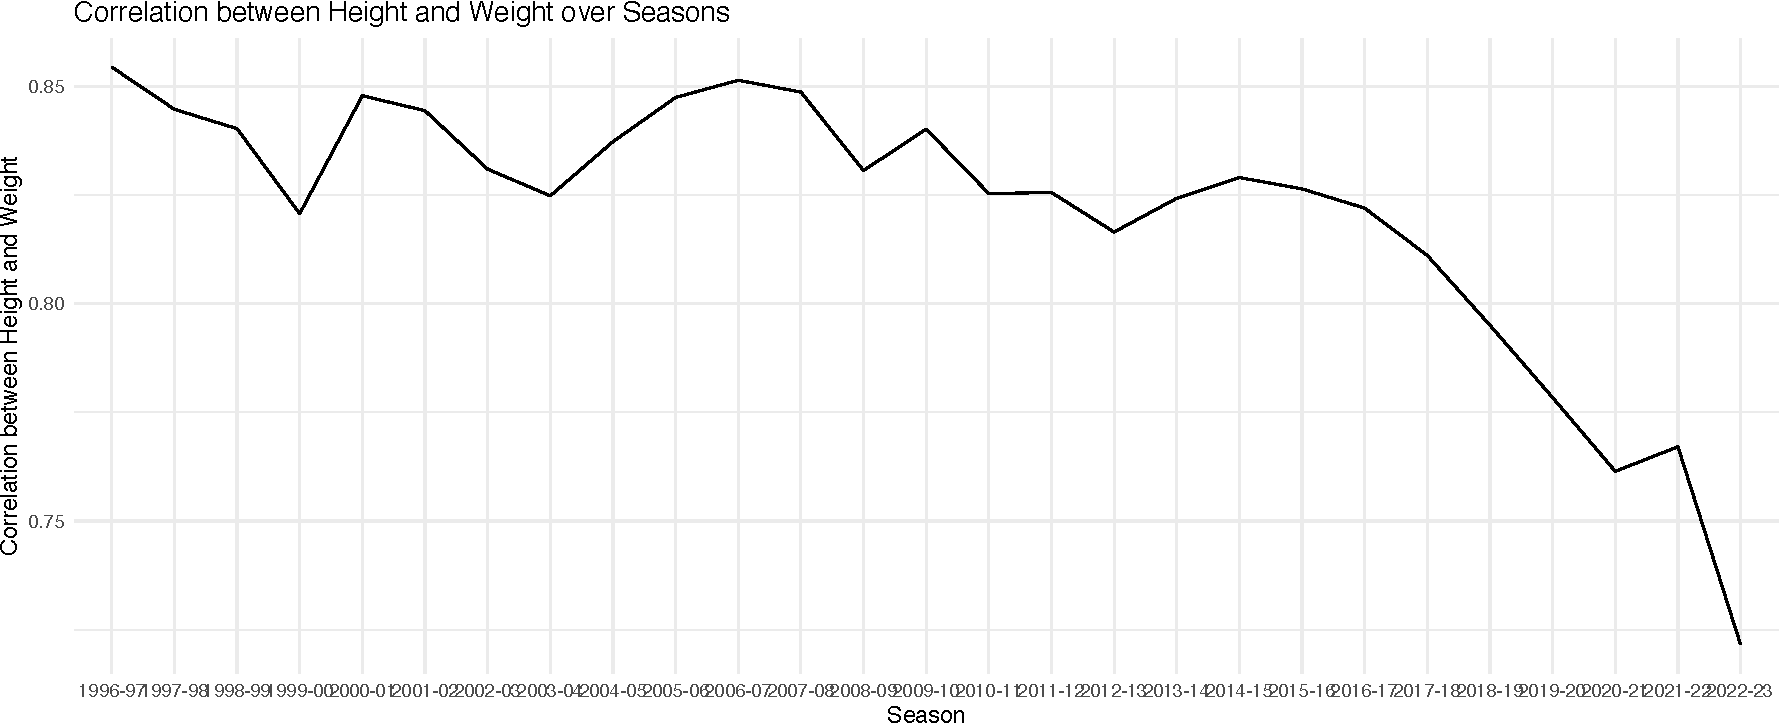
\includegraphics{NBA_Visualizing_files/figure-latex/unnamed-chunk-24-1.pdf}

\hypertarget{summary-from-4.2}{%
\section{Summary From 4.2}\label{summary-from-4.2}}

\begin{itemize}
\tightlist
\item
  A significant higher correlation between height and weight can be observed between season 1996-97 and 2009-10, suggesting a stronger relationship between a player's height and weight. This could have been due to the prevalence of taditional roles and the center-focused game styles, if we recall who were the most dominant players at that time (e.g., Shaquille O'Neal, Hakeem Olajuwon, Tim Duncan, Karl Malone, Dirk Nowitzki, Kevin Garnett)
\item
  Since the season 2009-10 , the correlation dips, suggesting a weaker relationship between height and weight. This potentially supports the hypothesis of ``position-less'' basketball becoming more prevalent, as players' roles become less defined by their physical attributes.
\end{itemize}

\hypertarget{clustering}{%
\chapter{Clustering}\label{clustering}}

\hypertarget{k-means-clustering-of-players}{%
\section{k-means Clustering Of Players}\label{k-means-clustering-of-players}}

To further investigate the transition in playing style and the trend toward position-less basketball, clustering analysis were conducted. This analysis used selected features including player height, weight, rebounds, assists, net rating, offensive rebounds, defensive rebounds, usage percentage, true shooting percentage, and assist percentage.

\textbf{What Data Was Included}

Given that more than 200 players participate in each NBA season and audiences generally remember high-scoring players, I applied specific criteria for more clear and understandable visualization results. For the selected seasons, only players who participated in more than 50 games and had an average score exceeding 10 points were included in the analysis.

\textbf{Selected Season}

\begin{itemize}
\item
  Based on the visualization in Section 4.2, a stronger correlation between height and weight (H/W) is evident between the seasons 1996-97 and 2009-10. This suggests a traditional, center-focused playing style, with a peak occurring in the 2000-01 season. To examine how player performance styles were clustered during periods when traditional styles dominated, we selected the 2000-01 and 2009-10 seasons.
\item
  NBA fans commonly believe that the ``small-ball center'' and ``three-point trend'' popularized by Stephen Curry's Golden State Warriors from 2015 to 2019 were catalysts for the transition in playing styles. To explore how player performance styles have evolved in more recent years, I selected the 2015-16 season and the most current season, 2022-2023.
\end{itemize}

\begin{Shaded}
\begin{Highlighting}[]
\NormalTok{nba\_selected\_season }\OtherTok{\textless{}{-}}\NormalTok{ nba[(}\FunctionTok{which}\NormalTok{(nba}\SpecialCharTok{$}\NormalTok{season }\SpecialCharTok{==}
    \StringTok{"2022{-}23"}\NormalTok{)), ]}
\NormalTok{nba\_selected\_season }\OtherTok{\textless{}{-}}\NormalTok{ nba\_selected\_season[nba\_selected\_season}\SpecialCharTok{$}\NormalTok{pts }\SpecialCharTok{\textgreater{}}
    \DecValTok{10}\NormalTok{, ]}
\NormalTok{nba\_selected\_season }\OtherTok{\textless{}{-}}\NormalTok{ nba\_selected\_season[nba\_selected\_season}\SpecialCharTok{$}\NormalTok{gp }\SpecialCharTok{\textgreater{}}
    \DecValTok{50}\NormalTok{, ]}
\FunctionTok{rownames}\NormalTok{(nba\_selected\_season) }\OtherTok{\textless{}{-}}\NormalTok{ nba\_selected\_season}\SpecialCharTok{$}\NormalTok{player\_name}

\NormalTok{selected\_features }\OtherTok{\textless{}{-}} \FunctionTok{c}\NormalTok{(}\StringTok{"player\_height"}\NormalTok{,}
    \StringTok{"pts"}\NormalTok{, }\StringTok{"player\_weight"}\NormalTok{,}
    \StringTok{"reb"}\NormalTok{, }\StringTok{"ast"}\NormalTok{, }\StringTok{"net\_rating"}\NormalTok{,}
    \StringTok{"oreb\_pct"}\NormalTok{, }\StringTok{"dreb\_pct"}\NormalTok{,}
    \StringTok{"usg\_pct"}\NormalTok{, }\StringTok{"ts\_pct"}\NormalTok{,}
    \StringTok{"ast\_pct"}\NormalTok{)}
\NormalTok{nba\_for\_clustering }\OtherTok{\textless{}{-}}\NormalTok{ nba\_selected\_season }\SpecialCharTok{\%\textgreater{}\%}
    \FunctionTok{select}\NormalTok{(}\FunctionTok{all\_of}\NormalTok{(selected\_features))}

\NormalTok{df }\OtherTok{\textless{}{-}} \FunctionTok{as.data.frame}\NormalTok{(}\FunctionTok{scale}\NormalTok{(nba\_for\_clustering))}


\FunctionTok{fviz\_nbclust}\NormalTok{(df, kmeans,}
    \AttributeTok{method =} \StringTok{"wss"}\NormalTok{) }\SpecialCharTok{+}
    \FunctionTok{geom\_vline}\NormalTok{(}\AttributeTok{xintercept =} \DecValTok{7}\NormalTok{,}
        \AttributeTok{linetype =} \DecValTok{2}\NormalTok{)}
\end{Highlighting}
\end{Shaded}

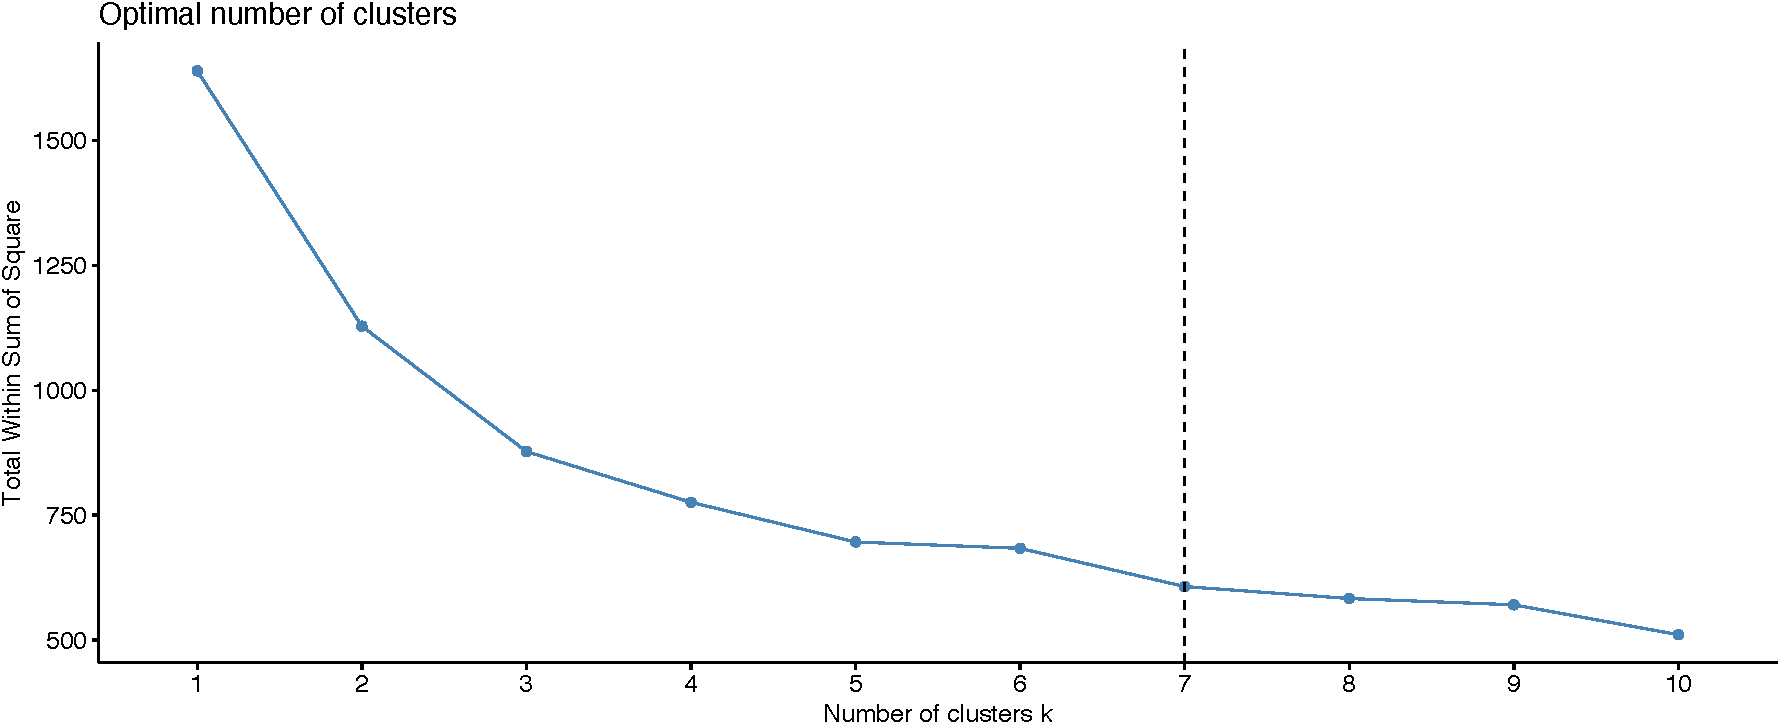
\includegraphics{NBA_Visualizing_files/figure-latex/unnamed-chunk-29-1.pdf}

\begin{Shaded}
\begin{Highlighting}[]
\FunctionTok{set.seed}\NormalTok{(}\DecValTok{123}\NormalTok{)}
\NormalTok{km\_result }\OtherTok{\textless{}{-}} \FunctionTok{kmeans}\NormalTok{(df,}
    \AttributeTok{centers =} \DecValTok{7}\NormalTok{)}
\end{Highlighting}
\end{Shaded}

\begin{Shaded}
\begin{Highlighting}[]
\NormalTok{clustering\_23 }\OtherTok{\textless{}{-}} \FunctionTok{fviz\_cluster}\NormalTok{(km\_result,}
    \AttributeTok{data =}\NormalTok{ df, }\AttributeTok{ellipse.type =} \StringTok{"euclid"}\NormalTok{,}
    \AttributeTok{ellipse.level =} \FloatTok{0.5}\NormalTok{,}
    \AttributeTok{ellipse.ratio =} \FloatTok{0.8}\NormalTok{,}
    \AttributeTok{star.plot =} \ConstantTok{TRUE}\NormalTok{,}
    \AttributeTok{repel =} \ConstantTok{TRUE}\NormalTok{, }\AttributeTok{main =} \StringTok{"NBA 2022{-}2023"}\NormalTok{,}
    \AttributeTok{ggtheme =} \FunctionTok{theme\_minimal}\NormalTok{())}

\NormalTok{clustering\_23 }\OtherTok{\textless{}{-}}\NormalTok{ clustering\_23 }\SpecialCharTok{+}
    \FunctionTok{theme}\NormalTok{(}\AttributeTok{plot.title =} \FunctionTok{element\_text}\NormalTok{(}\AttributeTok{size =} \DecValTok{30}\NormalTok{,}
        \AttributeTok{face =} \StringTok{"italic"}\NormalTok{,}
        \AttributeTok{color =} \StringTok{"blue"}\NormalTok{,}
        \AttributeTok{hjust =} \FloatTok{0.5}\NormalTok{,}
        \AttributeTok{vjust =} \DecValTok{1}\NormalTok{, }\AttributeTok{angle =} \DecValTok{0}\NormalTok{,}
        \AttributeTok{lineheight =} \FloatTok{1.2}\NormalTok{))}
\end{Highlighting}
\end{Shaded}

\textbf{For season 2000-01}

\begin{Shaded}
\begin{Highlighting}[]
\FunctionTok{print}\NormalTok{(clustering\_01)}
\end{Highlighting}
\end{Shaded}

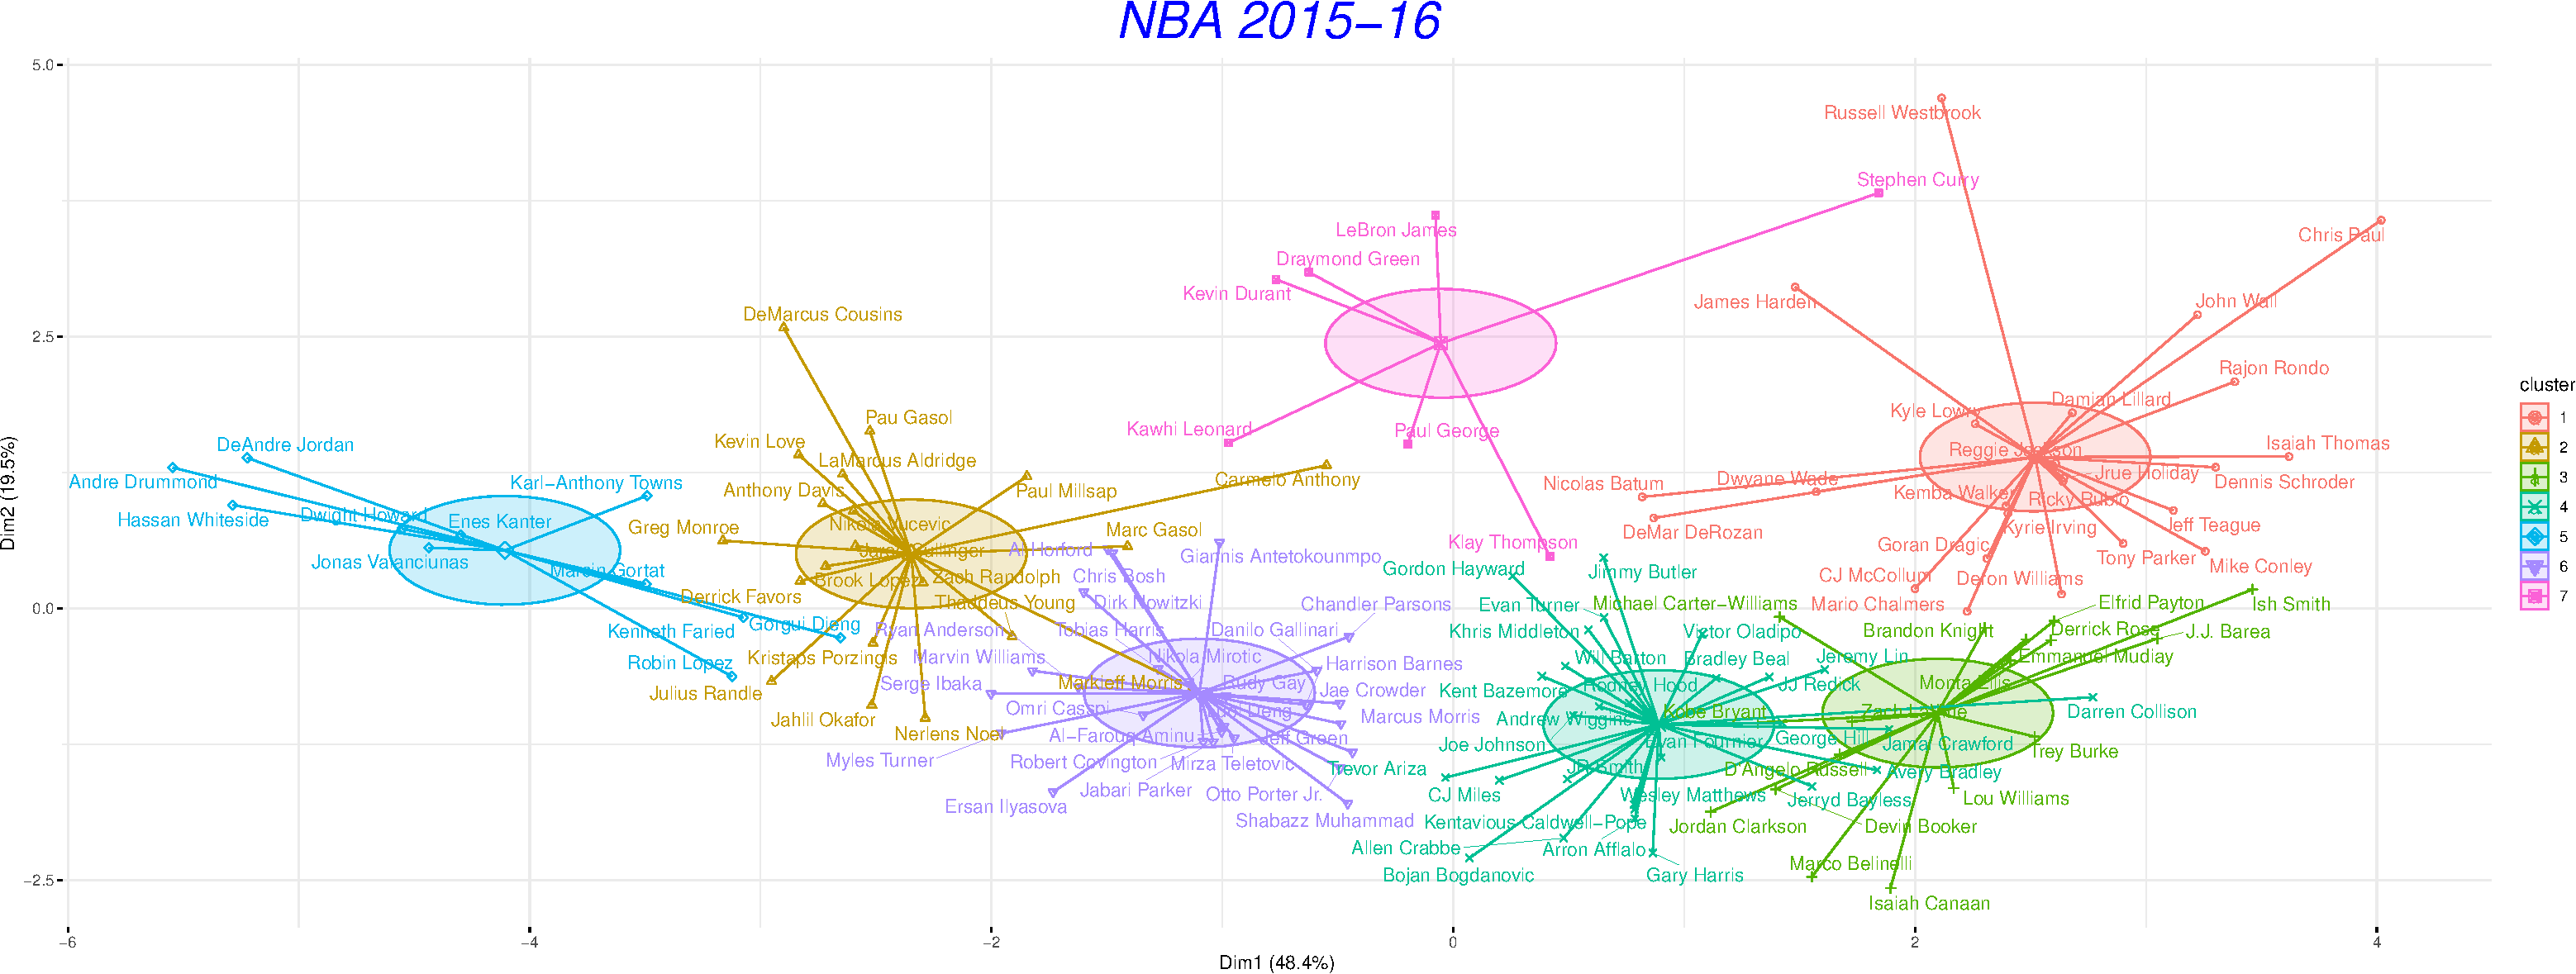
\includegraphics{NBA_Visualizing_files/figure-latex/unnamed-chunk-32-1.pdf}

\begin{Shaded}
\begin{Highlighting}[]
\FunctionTok{kable}\NormalTok{(mean\_values\_01)}
\end{Highlighting}
\end{Shaded}

\begin{tabular}{r|r|r|r|r|r}
\hline
cluster & player\_height & player\_weight & pts & reb & ast\\
\hline
1 & 200.3213 & 97.58276 & 23.06667 & 5.740000 & 4.360000\\
\hline
2 & 209.9733 & 116.49755 & 24.00000 & 11.300000 & 3.750000\\
\hline
3 & 209.4089 & 110.37405 & 14.03889 & 8.505556 & 1.650000\\
\hline
4 & 186.7568 & 84.94107 & 15.83158 & 3.736842 & 6.742105\\
\hline
5 & 198.7296 & 96.77839 & 13.65200 & 3.984000 & 2.472000\\
\hline
6 & 204.6705 & 107.38194 & 14.04211 & 6.105263 & 1.921053\\
\hline
7 & 191.5160 & 88.63188 & 16.12000 & 4.440000 & 6.420000\\
\hline
\end{tabular}

\textbf{For season 2009-10}

\begin{Shaded}
\begin{Highlighting}[]
\FunctionTok{print}\NormalTok{(clustering\_10)}
\end{Highlighting}
\end{Shaded}

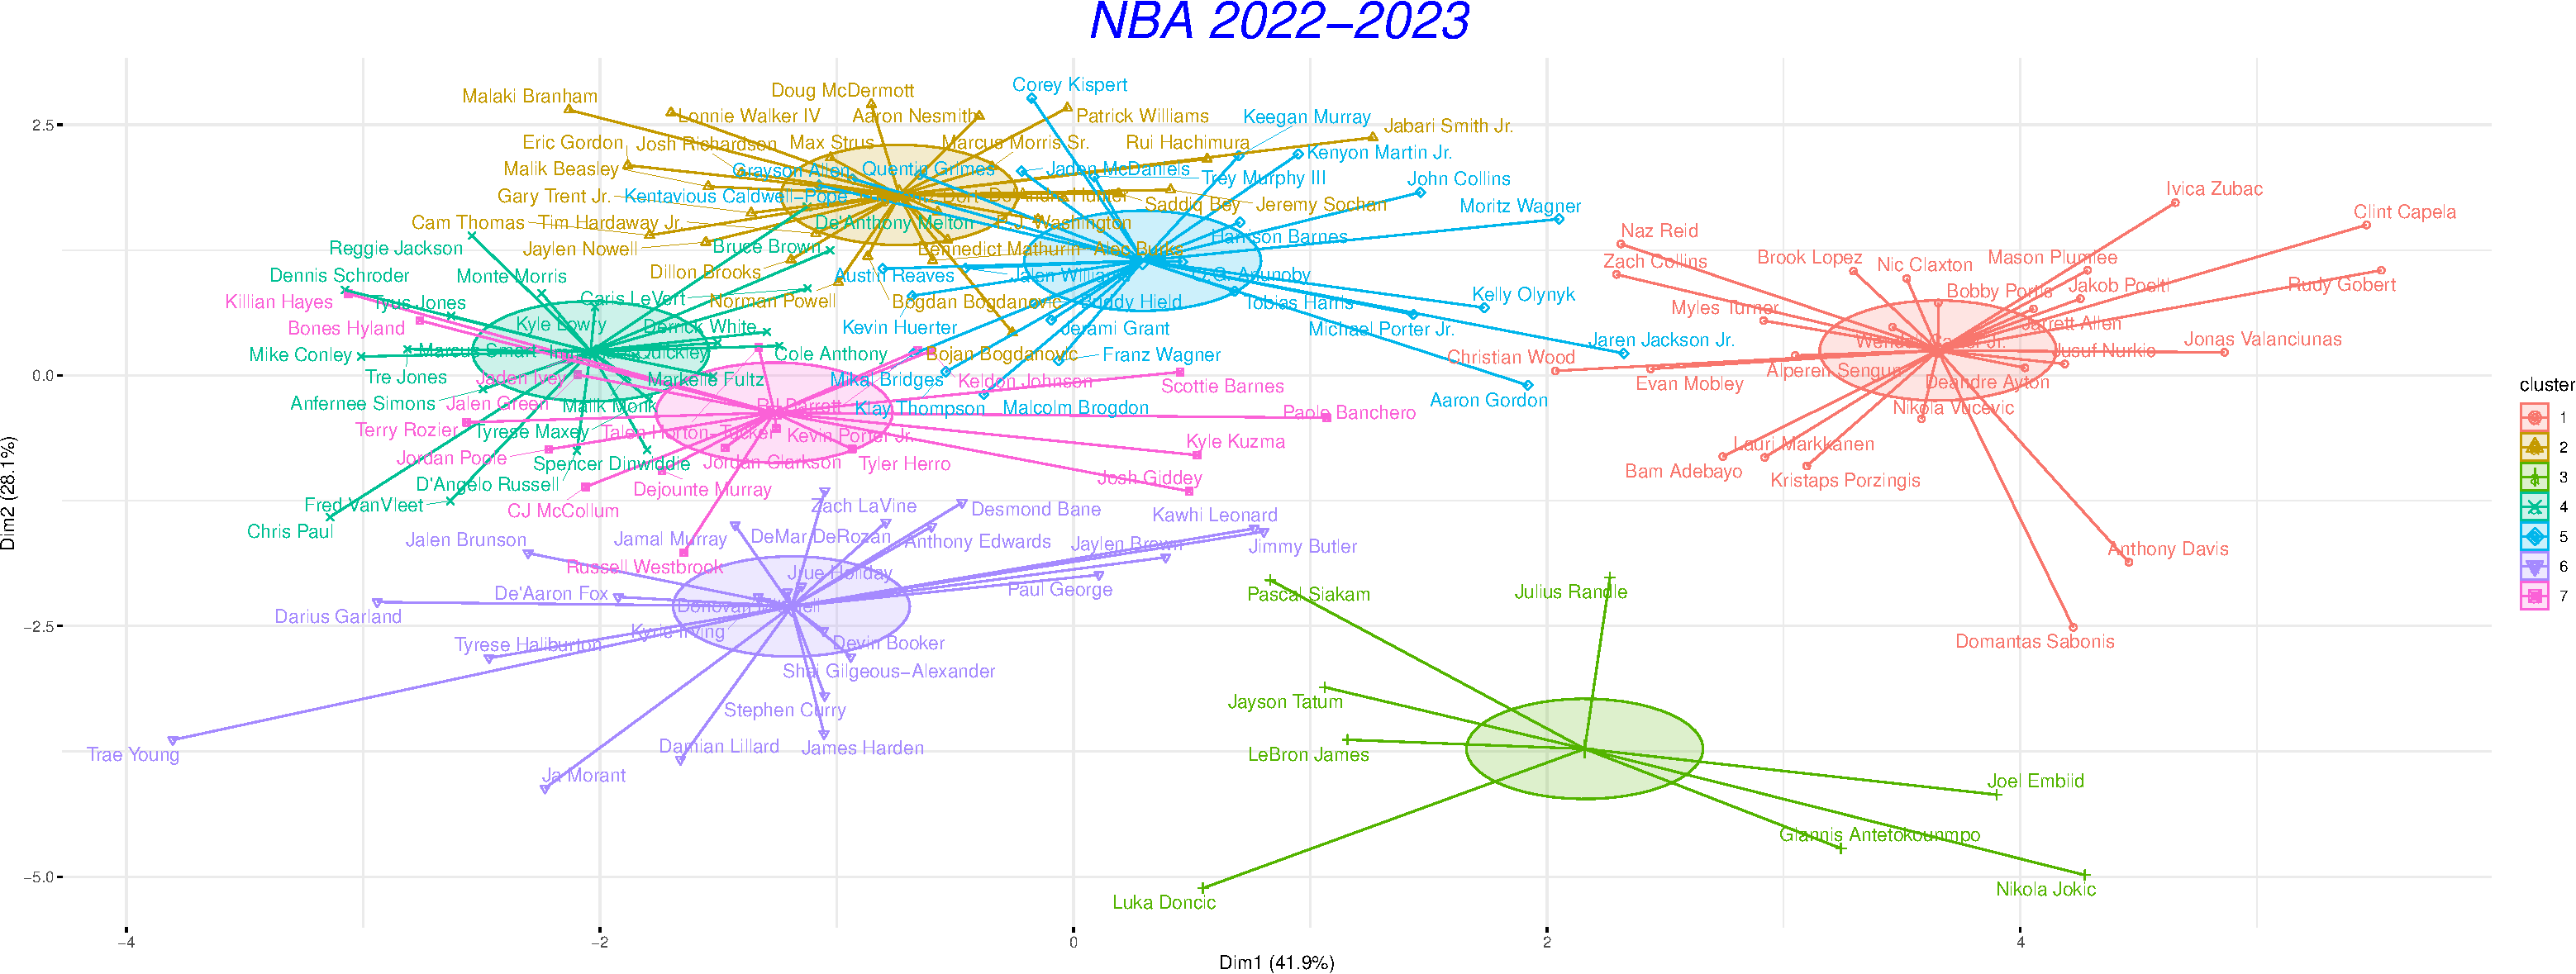
\includegraphics{NBA_Visualizing_files/figure-latex/unnamed-chunk-35-1.pdf}

\begin{Shaded}
\begin{Highlighting}[]
\FunctionTok{kable}\NormalTok{(mean\_values\_10)}
\end{Highlighting}
\end{Shaded}

\begin{tabular}{r|r|r|r|r|r}
\hline
cluster & player\_height & player\_weight & pts & reb & ast\\
\hline
1 & 192.5320 & 92.16989 & 17.78000 & 4.920000 & 9.800000\\
\hline
2 & 210.0792 & 117.59373 & 16.15000 & 9.754167 & 1.991667\\
\hline
3 & 187.4253 & 84.94107 & 14.20526 & 2.705263 & 4.673684\\
\hline
4 & 195.1789 & 93.79805 & 19.55789 & 4.378947 & 5.252632\\
\hline
5 & 206.3262 & 106.50689 & 15.16923 & 5.715385 & 1.834615\\
\hline
6 & 193.9471 & 91.36639 & 13.10714 & 2.964286 & 2.650000\\
\hline
7 & 205.5446 & 107.67576 & 14.13462 & 6.519231 & 2.338462\\
\hline
\end{tabular}

\textbf{For season 2015-16}

\begin{Shaded}
\begin{Highlighting}[]
\FunctionTok{print}\NormalTok{(clustering\_16)}
\end{Highlighting}
\end{Shaded}

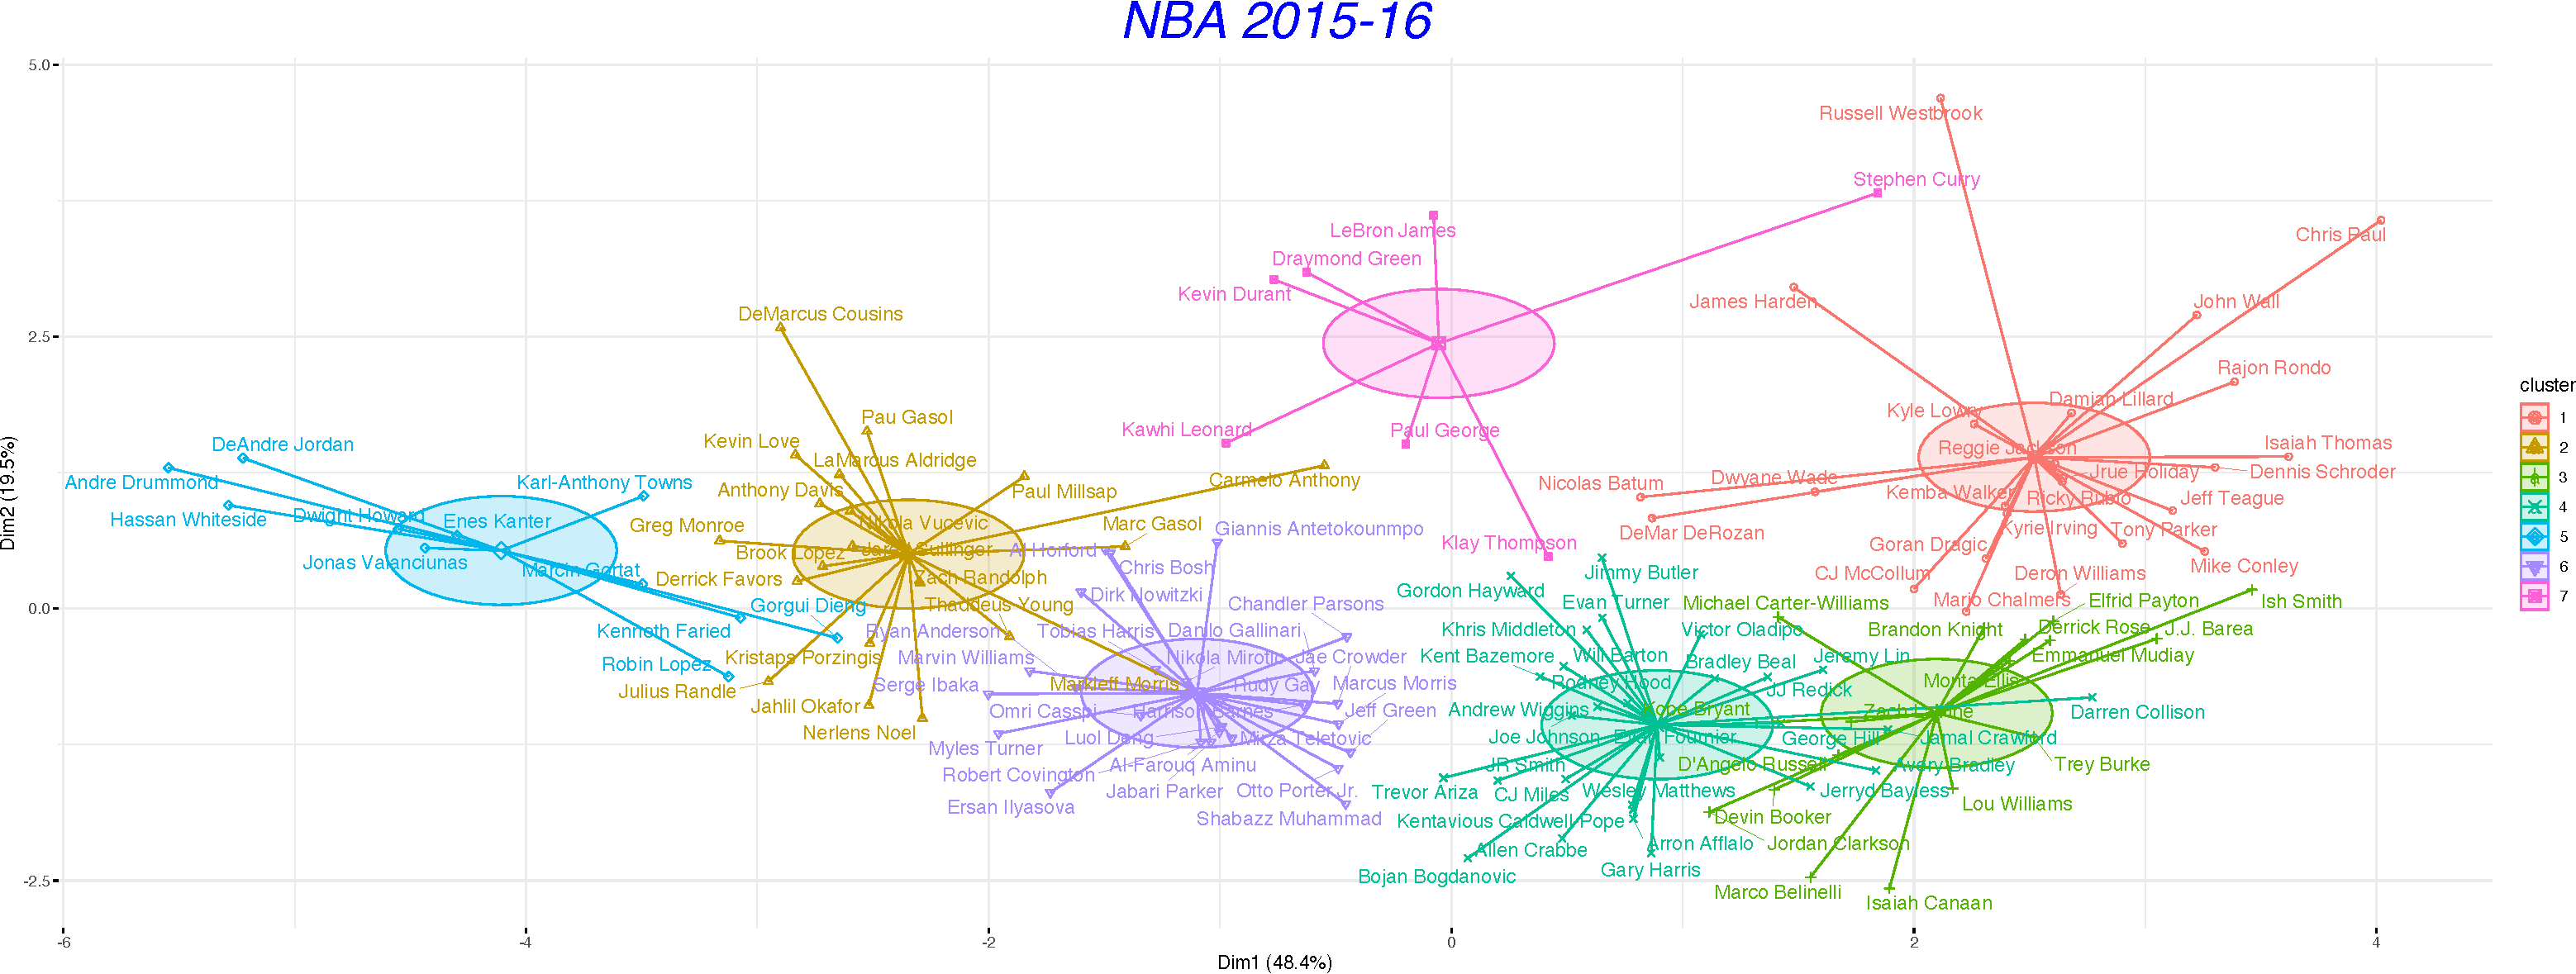
\includegraphics{NBA_Visualizing_files/figure-latex/unnamed-chunk-38-1.pdf}

\begin{Shaded}
\begin{Highlighting}[]
\FunctionTok{kable}\NormalTok{(mean\_values\_16)}
\end{Highlighting}
\end{Shaded}

\begin{tabular}{r|r|r|r|r|r}
\hline
cluster & player\_height & player\_weight & pts & reb & ast\\
\hline
1 & 189.7592 & 88.50714 & 17.87917 & 4.016667 & 6.491667\\
\hline
2 & 209.5500 & 114.50930 & 16.73000 & 8.585000 & 2.370000\\
\hline
3 & 191.5459 & 87.30312 & 13.50000 & 3.147059 & 3.817647\\
\hline
4 & 196.7593 & 94.16894 & 14.13929 & 3.557143 & 2.671429\\
\hline
5 & 211.0509 & 114.71754 & 13.36364 & 10.263636 & 1.145455\\
\hline
6 & 206.3262 & 104.76231 & 13.67692 & 5.723077 & 1.788461\\
\hline
7 & 201.0229 & 102.05820 & 23.42857 & 6.871429 & 4.957143\\
\hline
\end{tabular}

\textbf{For season 2022-23}

\begin{Shaded}
\begin{Highlighting}[]
\FunctionTok{print}\NormalTok{(clustering\_23)}
\end{Highlighting}
\end{Shaded}

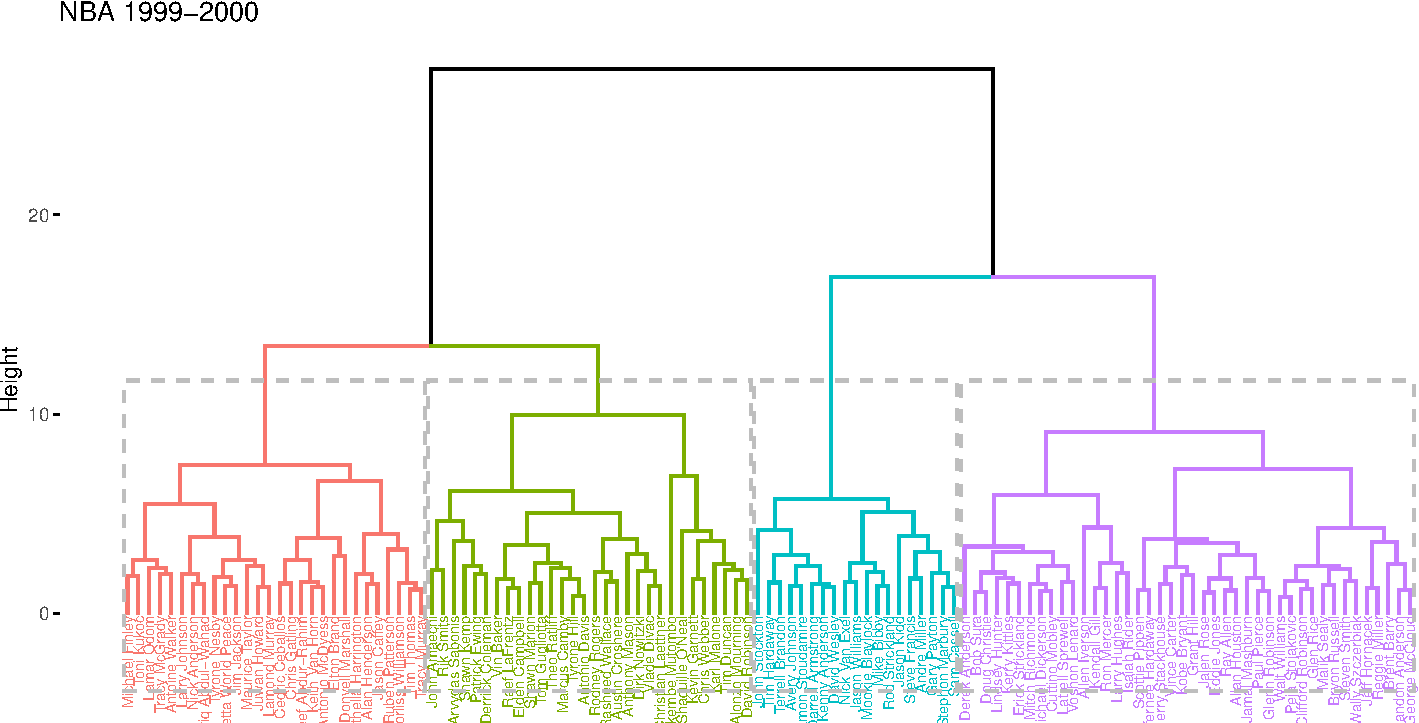
\includegraphics{NBA_Visualizing_files/figure-latex/unnamed-chunk-41-1.pdf}

\begin{Shaded}
\begin{Highlighting}[]
\FunctionTok{kable}\NormalTok{(mean\_values\_23)}
\end{Highlighting}
\end{Shaded}

\begin{tabular}{r|r|r|r|r|r}
\hline
cluster & player\_height & player\_weight & pts & reb & ast\\
\hline
1 & 211.3280 & 113.25285 & 15.90000 & 9.196000 & 2.352000\\
\hline
2 & 197.4615 & 97.10229 & 13.09259 & 3.555556 & 1.855556\\
\hline
3 & 206.6925 & 112.09392 & 28.67500 & 9.662500 & 6.125000\\
\hline
4 & 189.2300 & 88.18241 & 13.73182 & 3.427273 & 5.009091\\
\hline
5 & 201.2462 & 98.91795 & 14.81154 & 4.538462 & 2.276923\\
\hline
6 & 193.2609 & 92.27639 & 24.90000 & 4.917391 & 6.239130\\
\hline
7 & 195.5800 & 92.41340 & 18.14737 & 4.826316 & 4.700000\\
\hline
\end{tabular}

\hypertarget{summary-from-the-clustering}{%
\section{Summary From the Clustering}\label{summary-from-the-clustering}}

\textbf{H1 Versatility \& Position-less Basketball}

\begin{itemize}
\tightlist
\item
  2000-01 Season: players are more dispersed, suggesting a distinct division between positions based on physical attributes like height and weight. For example:

  \begin{itemize}
  \tightlist
  \item
    Traditional Centers: players around 7 feet tall and weighing between 250-300 lbs are prominent. These athletes typically represent traditional centers prevalent during this era (e.g., Tim Duncan, Karl Malone, Kevin Garnett, Dirk Nowitzki, Chris Webber, Shaquille O'Neal).
  \item
    Guards: athletes with heights ranging from 6'3'' to 6'6'' and weights between 180-210 lbs form distinct clusters, representing the roles of shooting and point guards.
  \end{itemize}
\item
  2009-10 Season: despite the strong correlation between height and weight suggested by Visualization 4.2, players like LeBron James and Dwyane Wade begin to lead the trend toward a more versatile playing style. LeBron James, for instance, while physically dominant enough to be considered a small forward, also demonstrates the skills and agility typical of guards. He can be grouped with well-known point guards like Steve Nash, Rajon Rondo, and Jason Kidd. On the other hand, players like Russell Westbrook, originally considered point guards, start taking on more scoring roles, leading them to be identified with scorers like Kobe Bryant and Carmelo Anthony. The diverse physical attributes within this scoring cluster make the transitional trend more apparent.
\item
  2015-16 Season: clusters start to merge, indicating the onset of the ``position-less'' trend. Players of various physical attributes now perform roles previously confined to specific positions. Draymond Green (6'6'', 230 lbs), for example, plays effectively as a point guard, power forward, and even center despite having the height of a traditional small forward. Additionally, dominant forwards who aren't traditional big men or guards but possess qualities of both are increasingly playing central roles (e.g., LeBron James, Kevin Durant, Kawhi Leonard).
\item
  2022-23 Season: clusters continue to converge, showcasing increasing versatility among players. Athletes with a narrow height range of 6'5'' to 6'10'' and weight range of 210-250 lbs are now playing multiple roles on the court---whether it's shooting, ball-handling, or post plays. Players like Luka Dončić, Giannis Antetokounmpo, LeBron James, and Nikola Jokić can be grouped in the same cluster, despite their varying physical sizes.
\end{itemize}

\textbf{H2 Evolution in Playing Style}

\begin{itemize}
\tightlist
\item
  2000-01 and 2009-10 Seasons: the dominance of players like Shaquille O'Neal and Tim Duncan indicates a game focused on the post and interior play, supporting the traditional center-focused style. At the same time, players like Kobe Bryant and Vince Carter, typically shooting guards, with a height-weight specification of around 6'6'' and 212 lbs, show the traditional divisions in playing roles.
\item
  2015-16 Season: with players like Stephen Curry and LeBron James leading the clusters from 2010 to 2020, it's evident that the style has evolved to prioritize agility, shooting range, and versatility. The game sees a rise in sharpshooters and versatile players. Stephen Curry (6'2'', 185 lbs) stands out with his unparalleled three-point shooting prowess.

  \begin{itemize}
  \tightlist
  \item
    LeBron James (6'9'', 250 lbs) is a classic example of versatility. Though traditionally a forward, players like him and Draymond Green can handle the ball and pass, and effectively play the defense role as either a forward, guard, or center, embodying the essence of position-less basketball.
  \end{itemize}
\item
  2022-23 Season: The domiannce of players like Giannis Antetokounmpo and Nikola Jokić who is traditionally regarded as big player, showcasing the prominent role in ball handling, pass, and play-making like a point guard. Meanwhile, player like Luka Dončić, standing at 6'7'' and weighing around 230 lbs, is a prime example of the modern player with a forward style medium-height but can lead the role of play-making and also play inside well.
\end{itemize}

\hypertarget{hierachical-clustering}{%
\section{Hierachical Clustering}\label{hierachical-clustering}}

To present a more intuitive depiction of the nested groupings in player clustering results, and to illustrate the gradual changes and transitions between seasons, we conducted hierarchical clustering visualization. The results were consistent with previous findings.

\begin{Shaded}
\begin{Highlighting}[]
\NormalTok{result\_23 }\OtherTok{\textless{}{-}} \FunctionTok{dist}\NormalTok{(df,}
    \AttributeTok{method =} \StringTok{"euclidean"}\NormalTok{)}
\NormalTok{result\_hc }\OtherTok{\textless{}{-}} \FunctionTok{hclust}\NormalTok{(}\AttributeTok{d =}\NormalTok{ result\_23,}
    \AttributeTok{method =} \StringTok{"ward.D2"}\NormalTok{)}
\FunctionTok{fviz\_dend}\NormalTok{(result\_hc,}
    \AttributeTok{k =} \DecValTok{4}\NormalTok{, }\AttributeTok{cex =} \FloatTok{0.5}\NormalTok{,}
    \AttributeTok{color\_labels\_by\_k =} \ConstantTok{TRUE}\NormalTok{,}
    \AttributeTok{main =} \StringTok{"NBA 2022{-}2023"}\NormalTok{,}
    \AttributeTok{rect =} \ConstantTok{TRUE}\NormalTok{)}
\end{Highlighting}
\end{Shaded}

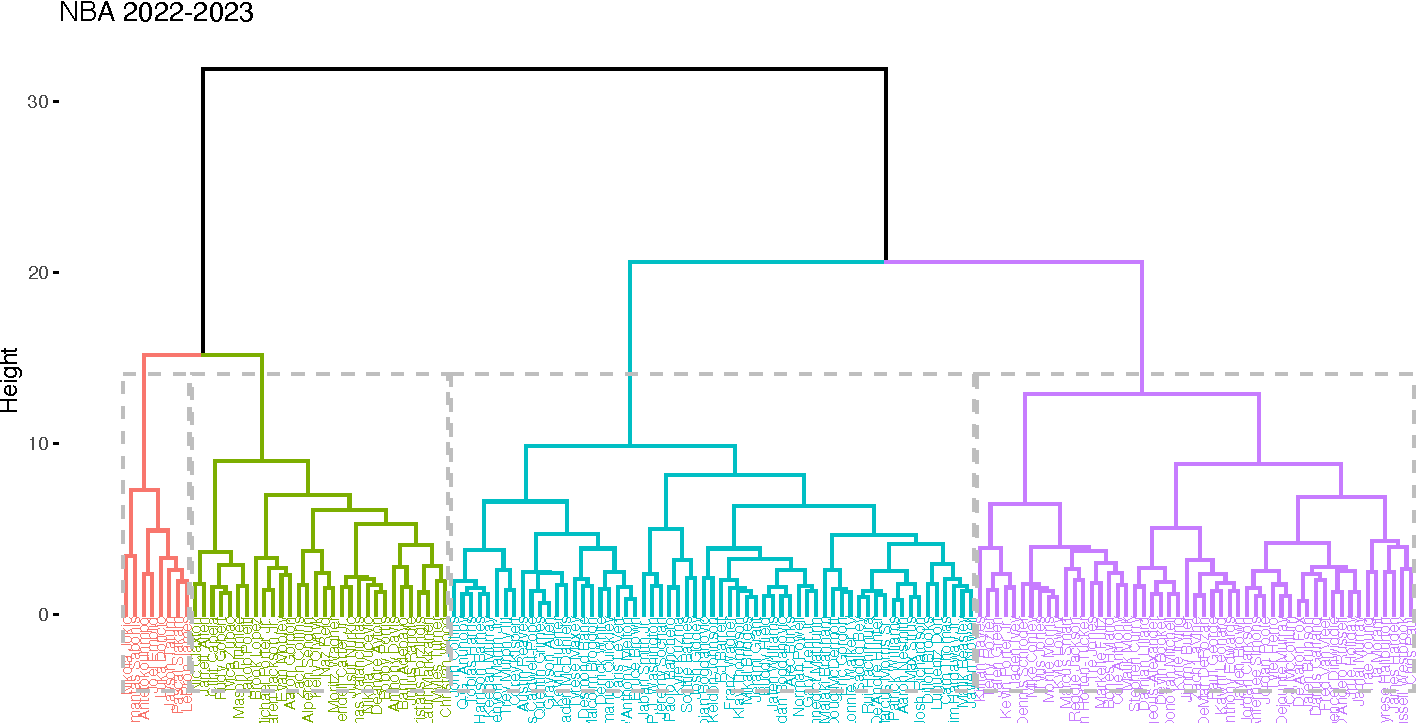
\includegraphics{NBA_Visualizing_files/figure-latex/unnamed-chunk-45-1.pdf}

\begin{Shaded}
\begin{Highlighting}[]
\FunctionTok{fviz\_dend}\NormalTok{(result\_hc\_01,}
    \AttributeTok{k =} \DecValTok{4}\NormalTok{, }\AttributeTok{cex =} \FloatTok{0.5}\NormalTok{,}
    \AttributeTok{color\_labels\_by\_k =} \ConstantTok{TRUE}\NormalTok{,}
    \AttributeTok{main =} \StringTok{"NBA 2000{-}2001"}\NormalTok{,}
    \AttributeTok{rect =} \ConstantTok{TRUE}\NormalTok{)}
\end{Highlighting}
\end{Shaded}

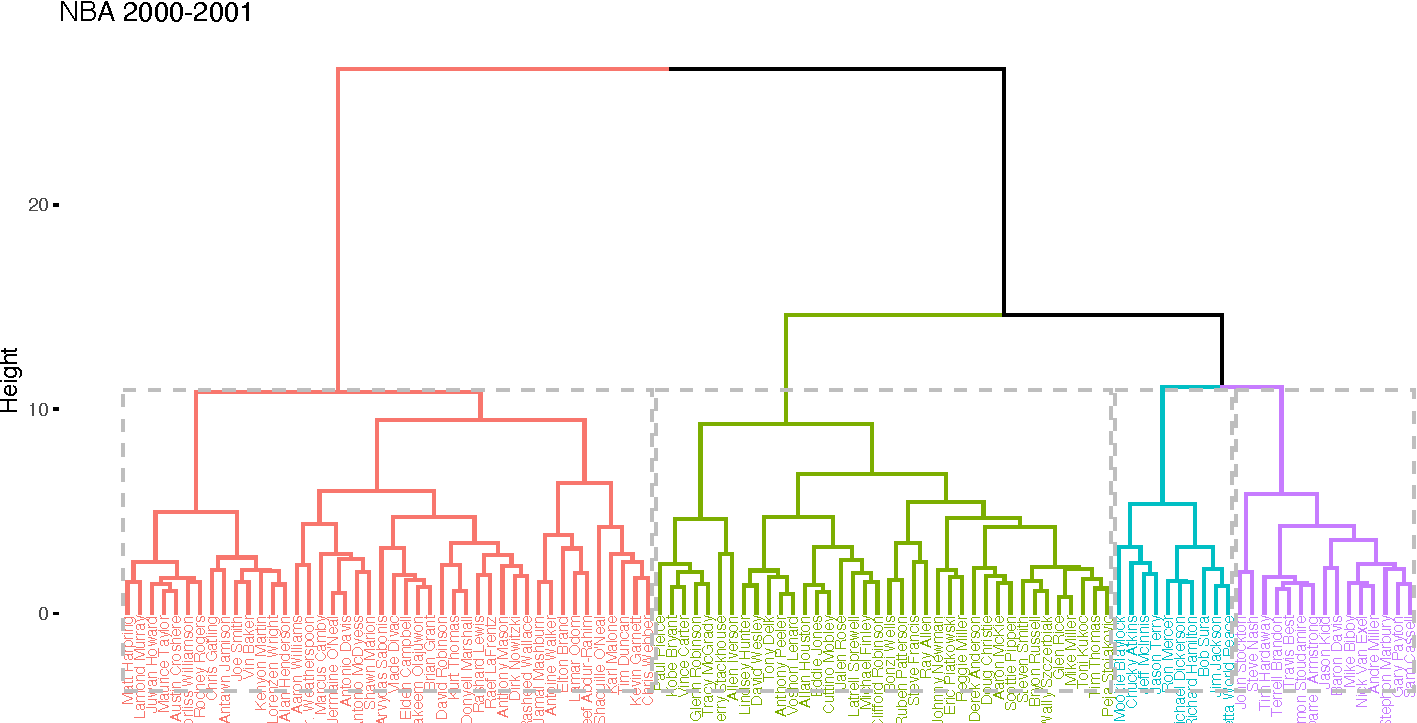
\includegraphics{NBA_Visualizing_files/figure-latex/unnamed-chunk-46-1.pdf}

\begin{Shaded}
\begin{Highlighting}[]
\FunctionTok{fviz\_dend}\NormalTok{(result\_hc\_10,}
    \AttributeTok{k =} \DecValTok{4}\NormalTok{, }\AttributeTok{cex =} \FloatTok{0.5}\NormalTok{,}
    \AttributeTok{color\_labels\_by\_k =} \ConstantTok{TRUE}\NormalTok{,}
    \AttributeTok{main =} \StringTok{"NBA 2009{-}2010"}\NormalTok{,}
    \AttributeTok{rect =} \ConstantTok{TRUE}\NormalTok{)}
\end{Highlighting}
\end{Shaded}

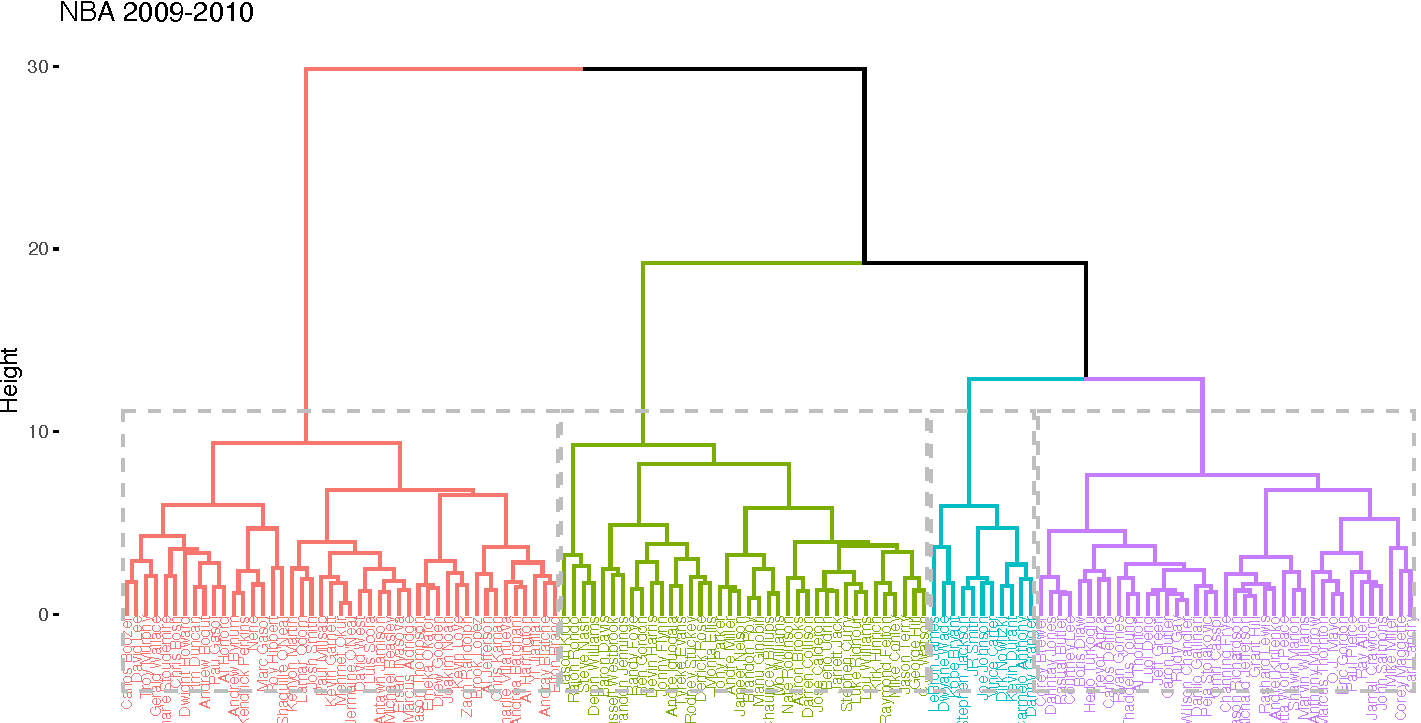
\includegraphics{NBA_Visualizing_files/figure-latex/unnamed-chunk-46-2.pdf}

\begin{Shaded}
\begin{Highlighting}[]
\FunctionTok{fviz\_dend}\NormalTok{(result\_hc\_16,}
    \AttributeTok{k =} \DecValTok{4}\NormalTok{, }\AttributeTok{cex =} \FloatTok{0.5}\NormalTok{,}
    \AttributeTok{color\_labels\_by\_k =} \ConstantTok{TRUE}\NormalTok{,}
    \AttributeTok{main =} \StringTok{"NBA 2015{-}2016"}\NormalTok{,}
    \AttributeTok{rect =} \ConstantTok{TRUE}\NormalTok{)}
\end{Highlighting}
\end{Shaded}

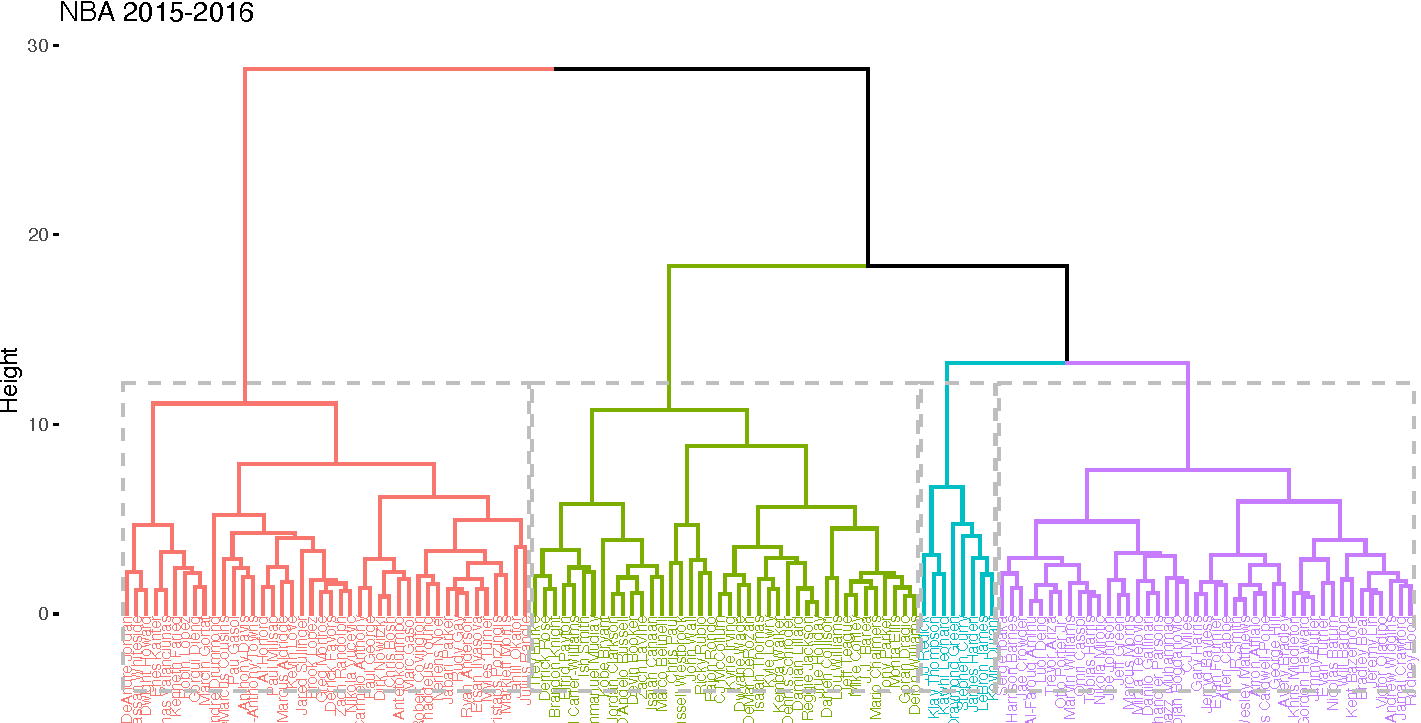
\includegraphics{NBA_Visualizing_files/figure-latex/unnamed-chunk-46-3.pdf}

\hypertarget{transition-of-nba-over-last-20-years}{%
\chapter{Transition of NBA Over Last 20 Years}\label{transition-of-nba-over-last-20-years}}

Over the past two decades, the NBA has undergone significant transformations, particularly in playing styles and player roles.

\hypertarget{versatility-position-less-basketball}{%
\section{Versatility \& Position-less Basketball}\label{versatility-position-less-basketball}}

The first ten year of this centry, the league showcased traditional player roles based on physical attributes. Centers like Shaquille O'Neal exemplified this trend with their dominance in the post. However, with the progression second ten year, there's a marked shift towards position-less basketball. Players like Stephen Curry, LeBron James, Giannis Antetokounmpo, Nikola Jokić exemplify this evolution. Initially known for his scoring, LeBron's game matured to include playmaking, passing, and even post play, adapting to the requirements of his team and the evolving nature of the NBA. This has paved the way for players who, regardless of their size, can perform multiple roles on the court.

\hypertarget{evolution-in-playing-style}{%
\section{Evolution in Playing Style}\label{evolution-in-playing-style}}

The NBA has transitioned from a center-focused play to a more perimeter-oriented game. This shift is evident when comparing the dominance of traditional centers in earlier seasons to the sharpshooting prowess of guards like Stephen Curry in later ones. The league has gravitated towards faster-paced, space-oriented offenses, capitalizing on three-point shots and versatile player skills.

\hypertarget{potential-future-trends}{%
\section{Potential Future Trends}\label{potential-future-trends}}

The increasing value of versatility suggests the NBA will continue to evolve towards an even faster, more skill-oriented game. Traditional roles might further blur, leading to players being valued more for their overall skill set rather than specific positional attributes.

As for physical attributes, while height will always be advantageous, it might not be the dominant factor in player evaluation. Agility, endurance, and skill versatility could become primary attributes scouts look for. For instance, players who, like LeBron, can adapt and reinvent their game will be highly prized. As teams prioritize speed and versatility, we may see an even more diverse range of player heights and weights, with an emphasis on adaptability both in play style and physical conditioning.

  \bibliography{book.bib,packages.bib}

\end{document}
